\documentclass[1p]{elsarticle_modified}
%\bibliographystyle{elsarticle-num}

%\usepackage[colorlinks]{hyperref}
%\usepackage{abbrmath_seonhwa} %\Abb, \Ascr, \Acal ,\Abf, \Afrak
\usepackage{amsfonts}
\usepackage{amssymb}
\usepackage{amsmath}
\usepackage{amsthm}
\usepackage{scalefnt}
\usepackage{amsbsy}
\usepackage{kotex}
\usepackage{caption}
\usepackage{subfig}
\usepackage{color}
\usepackage{graphicx}
\usepackage{xcolor} %% white, black, red, green, blue, cyan, magenta, yellow
\usepackage{float}
\usepackage{setspace}
\usepackage{hyperref}

\usepackage{tikz}
\usetikzlibrary{arrows}

\usepackage{multirow}
\usepackage{array} % fixed length table
\usepackage{hhline}

%%%%%%%%%%%%%%%%%%%%%
\makeatletter
\renewcommand*\env@matrix[1][\arraystretch]{%
	\edef\arraystretch{#1}%
	\hskip -\arraycolsep
	\let\@ifnextchar\new@ifnextchar
	\array{*\c@MaxMatrixCols c}}
\makeatother %https://tex.stackexchange.com/questions/14071/how-can-i-increase-the-line-spacing-in-a-matrix
%%%%%%%%%%%%%%%

\usepackage[normalem]{ulem}

\newcommand{\msout}[1]{\ifmmode\text{\sout{\ensuremath{#1}}}\else\sout{#1}\fi}
%SOURCE: \msout is \stkout macro in https://tex.stackexchange.com/questions/20609/strikeout-in-math-mode

\newcommand{\cancel}[1]{
	\ifmmode
	{\color{red}\msout{#1}}
	\else
	{\color{red}\sout{#1}}
	\fi
}

\newcommand{\add}[1]{
	{\color{blue}\uwave{#1}}
}

\newcommand{\replace}[2]{
	\ifmmode
	{\color{red}\msout{#1}}{\color{blue}\uwave{#2}}
	\else
	{\color{red}\sout{#1}}{\color{blue}\uwave{#2}}
	\fi
}

\newcommand{\Sol}{\mathcal{S}} %segment
\newcommand{\D}{D} %diagram
\newcommand{\A}{\mathcal{A}} %arc


%%%%%%%%%%%%%%%%%%%%%%%%%%%%%5 test

\def\sl{\operatorname{\textup{SL}}(2,\Cbb)}
\def\psl{\operatorname{\textup{PSL}}(2,\Cbb)}
\def\quan{\mkern 1mu \triangleright \mkern 1mu}

\theoremstyle{definition}
\newtheorem{thm}{Theorem}[section]
\newtheorem{prop}[thm]{Proposition}
\newtheorem{lem}[thm]{Lemma}
\newtheorem{ques}[thm]{Question}
\newtheorem{cor}[thm]{Corollary}
\newtheorem{defn}[thm]{Definition}
\newtheorem{exam}[thm]{Example}
\newtheorem{rmk}[thm]{Remark}
\newtheorem{alg}[thm]{Algorithm}

\newcommand{\I}{\sqrt{-1}}
\begin{document}

%\begin{frontmatter}
%
%\title{Boundary parabolic representations of knots up to 8 crossings}
%
%%% Group authors per affiliation:
%\author{Yunhi Cho} 
%\address{Department of Mathematics, University of Seoul, Seoul, Korea}
%\ead{yhcho@uos.ac.kr}
%
%
%\author{Seonhwa Kim} %\fnref{s_kim}}
%\address{Center for Geometry and Physics, Institute for Basic Science, Pohang, 37673, Korea}
%\ead{ryeona17@ibs.re.kr}
%
%\author{Hyuk Kim}
%\address{Department of Mathematical Sciences, Seoul National University, Seoul 08826, Korea}
%\ead{hyukkim@snu.ac.kr}
%
%\author{Seokbeom Yoon}
%\address{Department of Mathematical Sciences, Seoul National University, Seoul, 08826,  Korea}
%\ead{sbyoon15@snu.ac.kr}
%
%\begin{abstract}
%We find all boundary parabolic representation of knots up to 8 crossings.
%
%\end{abstract}
%\begin{keyword}
%    \MSC[2010] 57M25 
%\end{keyword}
%
%\end{frontmatter}

%\linenumbers
%\tableofcontents
%
\newcommand\colored[1]{\textcolor{white}{\rule[-0.35ex]{0.8em}{1.4ex}}\kern-0.8em\color{red} #1}%
%\newcommand\colored[1]{\textcolor{white}{ #1}\kern-2.17ex	\textcolor{white}{ #1}\kern-1.81ex	\textcolor{white}{ #1}\kern-2.15ex\color{red}#1	}

{\Large $\underline{12a_{0616}~(K12a_{0616})}$}

\setlength{\tabcolsep}{10pt}
\renewcommand{\arraystretch}{1.6}
\vspace{1cm}\begin{tabular}{m{100pt}>{\centering\arraybackslash}m{274pt}}
\multirow{5}{120pt}{
	\centering
	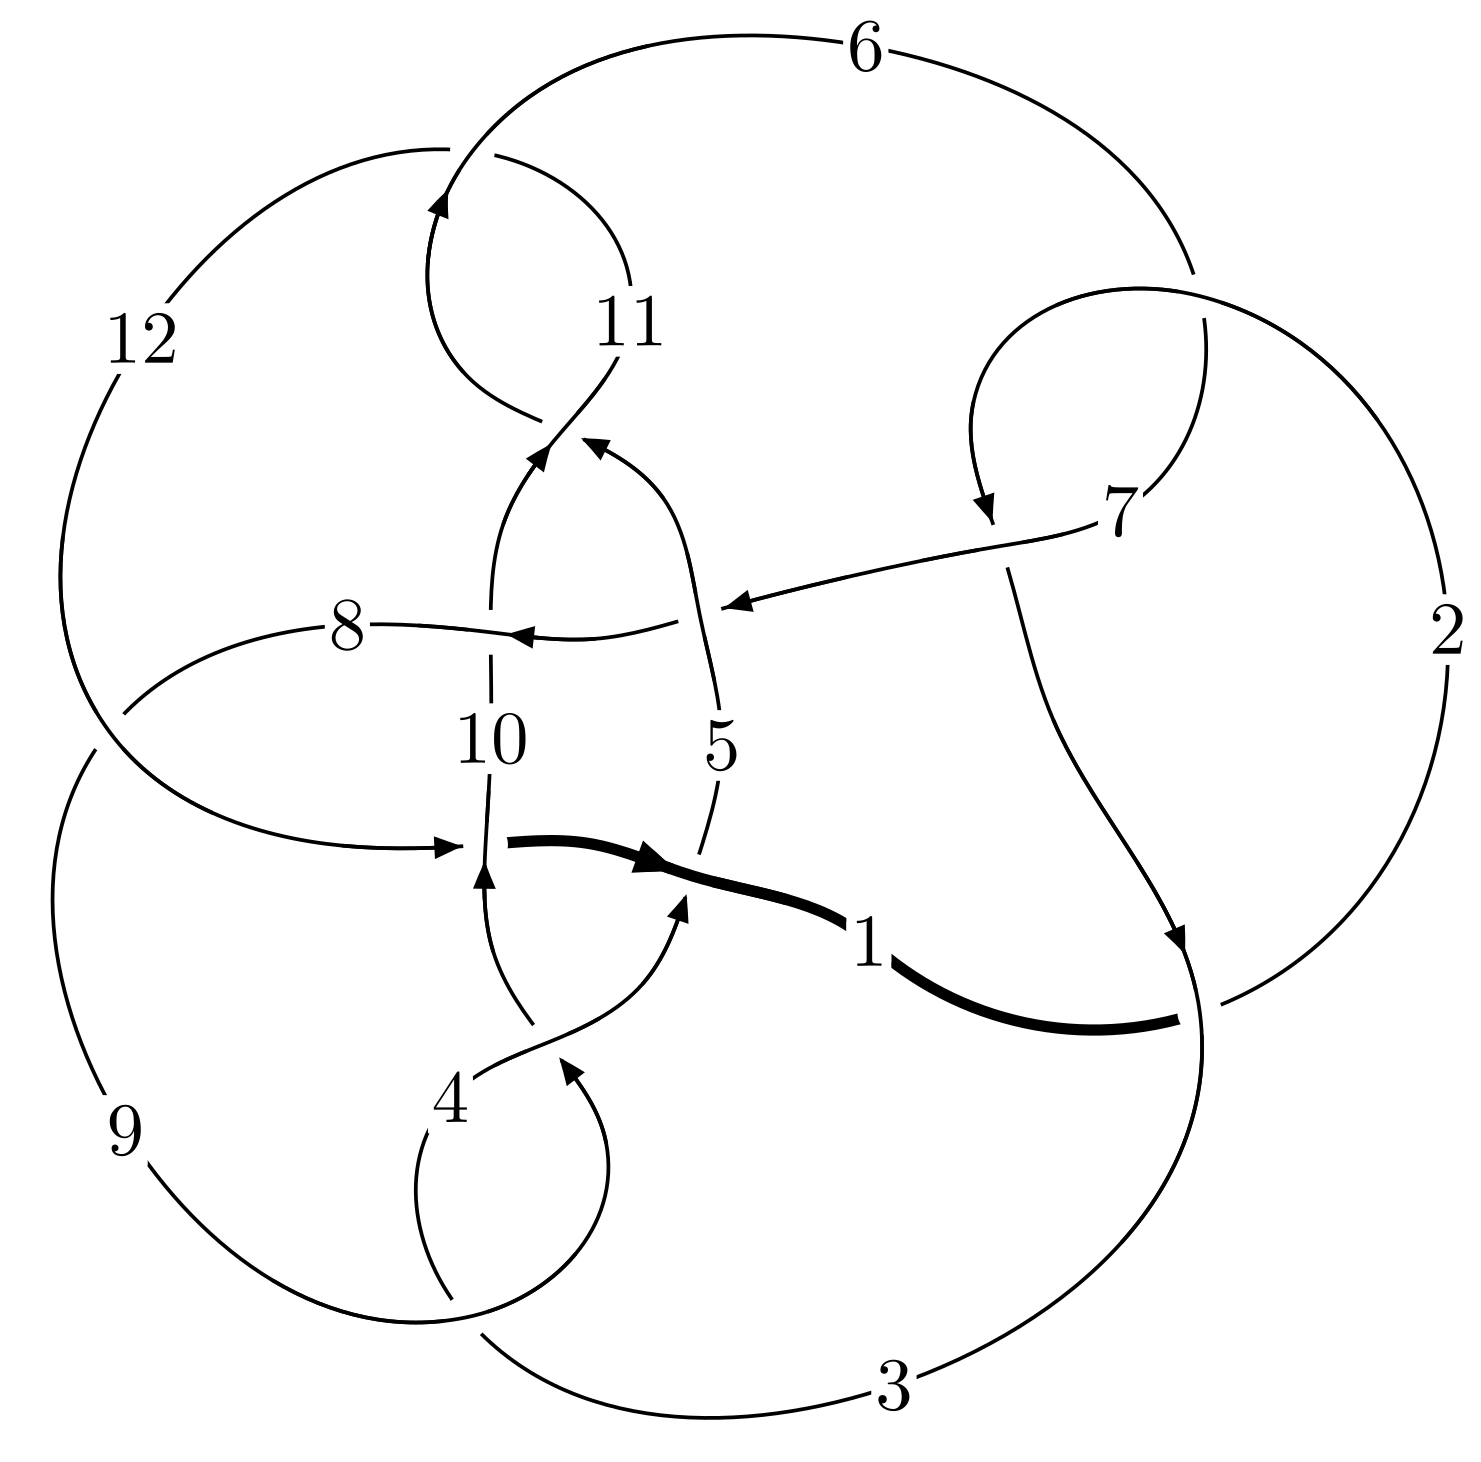
\includegraphics[width=112pt]{../../../GIT/diagram.site/Diagrams/png/1417_12a_0616.png}\\
\ \ \ A knot diagram\footnotemark}&
\allowdisplaybreaks
\textbf{Linearized knot diagam} \\
\cline{2-2}
 &
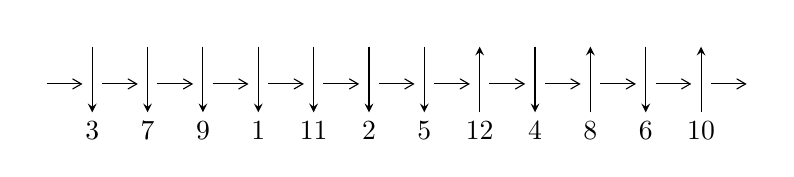
\begin{tikzpicture}[x=20pt, y=17pt]
	% nodes
	\node (C0) at (0, 0) {};
	\node (C1) at (1, 0) {};
	\node (C1U) at (1, +1) {};
	\node (C1D) at (1, -1) {3};

	\node (C2) at (2, 0) {};
	\node (C2U) at (2, +1) {};
	\node (C2D) at (2, -1) {7};

	\node (C3) at (3, 0) {};
	\node (C3U) at (3, +1) {};
	\node (C3D) at (3, -1) {9};

	\node (C4) at (4, 0) {};
	\node (C4U) at (4, +1) {};
	\node (C4D) at (4, -1) {1};

	\node (C5) at (5, 0) {};
	\node (C5U) at (5, +1) {};
	\node (C5D) at (5, -1) {11};

	\node (C6) at (6, 0) {};
	\node (C6U) at (6, +1) {};
	\node (C6D) at (6, -1) {2};

	\node (C7) at (7, 0) {};
	\node (C7U) at (7, +1) {};
	\node (C7D) at (7, -1) {5};

	\node (C8) at (8, 0) {};
	\node (C8U) at (8, +1) {};
	\node (C8D) at (8, -1) {12};

	\node (C9) at (9, 0) {};
	\node (C9U) at (9, +1) {};
	\node (C9D) at (9, -1) {4};

	\node (C10) at (10, 0) {};
	\node (C10U) at (10, +1) {};
	\node (C10D) at (10, -1) {8};

	\node (C11) at (11, 0) {};
	\node (C11U) at (11, +1) {};
	\node (C11D) at (11, -1) {6};

	\node (C12) at (12, 0) {};
	\node (C12U) at (12, +1) {};
	\node (C12D) at (12, -1) {10};
	\node (C13) at (13, 0) {};

	% arrows
	\draw[->,>={angle 60}]
	(C0) edge (C1) (C1) edge (C2) (C2) edge (C3) (C3) edge (C4) (C4) edge (C5) (C5) edge (C6) (C6) edge (C7) (C7) edge (C8) (C8) edge (C9) (C9) edge (C10) (C10) edge (C11) (C11) edge (C12) (C12) edge (C13) ;	\draw[->,>=stealth]
	(C1U) edge (C1D) (C2U) edge (C2D) (C3U) edge (C3D) (C4U) edge (C4D) (C5U) edge (C5D) (C6U) edge (C6D) (C7U) edge (C7D) (C8D) edge (C8U) (C9U) edge (C9D) (C10D) edge (C10U) (C11U) edge (C11D) (C12D) edge (C12U) ;
	\end{tikzpicture} \\
\hhline{~~} \\& 
\textbf{Solving Sequence} \\ \cline{2-2} 
 &
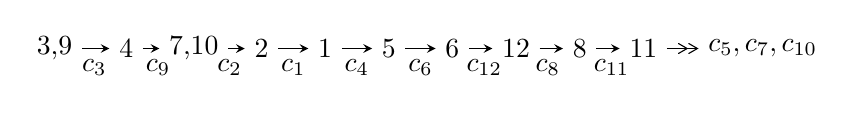
\begin{tikzpicture}[x=23pt, y=7pt]
	% node
	\node (A0) at (-1/8, 0) {3,9};
	\node (A1) at (1, 0) {4};
	\node (A2) at (33/16, 0) {7,10};
	\node (A3) at (25/8, 0) {2};
	\node (A4) at (33/8, 0) {1};
	\node (A5) at (41/8, 0) {5};
	\node (A6) at (49/8, 0) {6};
	\node (A7) at (57/8, 0) {12};
	\node (A8) at (65/8, 0) {8};
	\node (A9) at (73/8, 0) {11};
	\node (C1) at (1/2, -1) {$c_{3}$};
	\node (C2) at (3/2, -1) {$c_{9}$};
	\node (C3) at (21/8, -1) {$c_{2}$};
	\node (C4) at (29/8, -1) {$c_{1}$};
	\node (C5) at (37/8, -1) {$c_{4}$};
	\node (C6) at (45/8, -1) {$c_{6}$};
	\node (C7) at (53/8, -1) {$c_{12}$};
	\node (C8) at (61/8, -1) {$c_{8}$};
	\node (C9) at (69/8, -1) {$c_{11}$};
	\node (A10) at (11, 0) {$c_{5},c_{7},c_{10}$};

	% edge
	\draw[->,>=stealth]	
	(A0) edge (A1) (A1) edge (A2) (A2) edge (A3) (A3) edge (A4) (A4) edge (A5) (A5) edge (A6) (A6) edge (A7) (A7) edge (A8) (A8) edge (A9) ;
	\draw[->>,>={angle 60}]	
	(A9) edge (A10);
\end{tikzpicture} \\ 

\end{tabular} \\

\footnotetext{
The image of knot diagram is generated by the software ``\textbf{Draw programme}" developed by Andrew Bartholomew(\url{http://www.layer8.co.uk/maths/draw/index.htm\#Running-draw}), where we modified some parts for our purpose(\url{https://github.com/CATsTAILs/LinksPainter}).
}\phantom \\ \newline 
\centering \textbf{Ideals for irreducible components\footnotemark of $X_{\text{par}}$} 
 
\begin{align*}
I^u_{1}&=\langle 
1.87565\times10^{37} u^{44}+2.88467\times10^{37} u^{43}+\cdots+1.79366\times10^{38} b-2.28855\times10^{38},\\
\phantom{I^u_{1}}&\phantom{= \langle  }-6.32625\times10^{36} u^{44}-1.60162\times10^{37} u^{43}+\cdots+1.79366\times10^{38} a+2.72634\times10^{38},\\
\phantom{I^u_{1}}&\phantom{= \langle  }u^{45}-16 u^{43}+\cdots+8 u+8\rangle \\
I^u_{2}&=\langle 
1.05402\times10^{619} u^{135}-1.25591\times10^{619} u^{134}+\cdots+1.02383\times10^{619} b-5.96436\times10^{620},\\
\phantom{I^u_{2}}&\phantom{= \langle  }-1.18864\times10^{621} u^{135}+2.70367\times10^{621} u^{134}+\cdots+9.11212\times10^{620} a+2.71391\times10^{623},\\
\phantom{I^u_{2}}&\phantom{= \langle  }u^{136}- u^{135}+\cdots-1494 u-89\rangle \\
I^u_{3}&=\langle 
- u^{10}+4 u^8-6 u^6+u^5+3 u^4-2 u^3+b+u-1,\;u^{10}- u^9-5 u^8+4 u^7+9 u^6-6 u^5-5 u^4+3 u^3-2 u^2+a+2,\\
\phantom{I^u_{3}}&\phantom{= \langle  }u^{11}-5 u^9+9 u^7- u^6-5 u^5+3 u^4-2 u^3-2 u^2+2 u-1\rangle \\
I^u_{4}&=\langle 
-1.69543\times10^{27} u^{37}+1.23907\times10^{27} u^{36}+\cdots+5.29826\times10^{24} b+1.95738\times10^{28},\\
\phantom{I^u_{4}}&\phantom{= \langle  }-1.69867\times10^{27} u^{37}+1.42937\times10^{27} u^{36}+\cdots+5.29826\times10^{24} a+1.47189\times10^{28},\;u^{38}-7 u^{36}+\cdots-8 u-8\rangle \\
\\
\end{align*}
\raggedright * 4 irreducible components of $\dim_{\mathbb{C}}=0$, with total 230 representations.\\
\footnotetext{All coefficients of polynomials are rational numbers. But the coefficients are sometimes approximated in decimal forms when there is not enough margin.}
\newpage
\renewcommand{\arraystretch}{1}
\centering \section*{I. $I^u_{1}= \langle 1.88\times10^{37} u^{44}+2.88\times10^{37} u^{43}+\cdots+1.79\times10^{38} b-2.29\times10^{38},\;-6.33\times10^{36} u^{44}-1.60\times10^{37} u^{43}+\cdots+1.79\times10^{38} a+2.73\times10^{38},\;u^{45}-16 u^{43}+\cdots+8 u+8 \rangle$}
\flushleft \textbf{(i) Arc colorings}\\
\begin{tabular}{m{7pt} m{180pt} m{7pt} m{180pt} }
\flushright $a_{3}=$&$\begin{pmatrix}1\\0\end{pmatrix}$ \\
\flushright $a_{9}=$&$\begin{pmatrix}0\\u\end{pmatrix}$ \\
\flushright $a_{4}=$&$\begin{pmatrix}1\\u^2\end{pmatrix}$ \\
\flushright $a_{7}=$&$\begin{pmatrix}0.0352702 u^{44}+0.0892935 u^{43}+\cdots+0.195710 u-1.51999\\-0.104571 u^{44}-0.160827 u^{43}+\cdots+2.45646 u+1.27591\end{pmatrix}$ \\
\flushright $a_{10}=$&$\begin{pmatrix}- u\\- u^3+u\end{pmatrix}$ \\
\flushright $a_{2}=$&$\begin{pmatrix}-0.0844913 u^{44}-0.185903 u^{43}+\cdots-0.0125427 u+2.53802\\0.127167 u^{44}+0.359944 u^{43}+\cdots-2.61521 u-2.76088\end{pmatrix}$ \\
\flushright $a_{1}=$&$\begin{pmatrix}0.0426760 u^{44}+0.174042 u^{43}+\cdots-2.62775 u-0.222856\\0.127167 u^{44}+0.359944 u^{43}+\cdots-2.61521 u-2.76088\end{pmatrix}$ \\
\flushright $a_{5}=$&$\begin{pmatrix}0.100777 u^{44}+0.0808879 u^{43}+\cdots-1.02805 u+0.638734\\-0.186080 u^{44}-0.0634539 u^{43}+\cdots+0.572085 u+0.149929\end{pmatrix}$ \\
\flushright $a_{6}=$&$\begin{pmatrix}-0.266430 u^{44}-0.128670 u^{43}+\cdots+1.92246 u-0.109400\\-0.0702591 u^{44}+0.300563 u^{43}+\cdots+0.746284 u-1.52508\end{pmatrix}$ \\
\flushright $a_{12}=$&$\begin{pmatrix}-0.0625033 u^{44}-0.153291 u^{43}+\cdots+0.239176 u+1.76637\\0.128670 u^{44}+0.318945 u^{43}+\cdots-2.02204 u-2.13144\end{pmatrix}$ \\
\flushright $a_{8}=$&$\begin{pmatrix}0.130212 u^{44}+0.255879 u^{43}+\cdots-3.03747 u-2.28189\\-0.111369 u^{44}-0.357286 u^{43}+\cdots+3.45797 u+1.82626\end{pmatrix}$ \\
\flushright $a_{11}=$&$\begin{pmatrix}0.0661668 u^{44}+0.165654 u^{43}+\cdots-1.78287 u-0.365073\\-0.171893 u^{44}+0.256339 u^{43}+\cdots-1.05904 u-2.69352\end{pmatrix}$\\&\end{tabular}
\flushleft \textbf{(ii) Obstruction class $= -1$}\\~\\
\flushleft \textbf{(iii) Cusp Shapes $= -0.795897 u^{44}-0.590986 u^{43}+\cdots+11.4411 u-4.15369$}\\~\\
\newpage\renewcommand{\arraystretch}{1}
\flushleft \textbf{(iv) u-Polynomials at the component}\newline \\
\begin{tabular}{m{50pt}|m{274pt}}
Crossings & \hspace{64pt}u-Polynomials at each crossing \\
\hline $$\begin{aligned}c_{1}\end{aligned}$$&$\begin{aligned}
&u^{45}+18 u^{44}+\cdots+380 u+16
\end{aligned}$\\
\hline $$\begin{aligned}c_{2},c_{6}\end{aligned}$$&$\begin{aligned}
&u^{45}-10 u^{44}+\cdots-42 u+4
\end{aligned}$\\
\hline $$\begin{aligned}c_{3},c_{5},c_{9}\\c_{11}\end{aligned}$$&$\begin{aligned}
&u^{45}-16 u^{43}+\cdots+8 u+8
\end{aligned}$\\
\hline $$\begin{aligned}c_{4},c_{7}\end{aligned}$$&$\begin{aligned}
&u^{45}-2 u^{44}+\cdots-40 u+7
\end{aligned}$\\
\hline $$\begin{aligned}c_{8}\end{aligned}$$&$\begin{aligned}
&u^{45}-24 u^{44}+\cdots-7732 u+1004
\end{aligned}$\\
\hline $$\begin{aligned}c_{10},c_{12}\end{aligned}$$&$\begin{aligned}
&u^{45}+2 u^{44}+\cdots+7 u+1
\end{aligned}$\\
\hline
\end{tabular}\\~\\
\newpage\renewcommand{\arraystretch}{1}
\flushleft \textbf{(v) Riley Polynomials at the component}\newline \\
\begin{tabular}{m{50pt}|m{274pt}}
Crossings & \hspace{64pt}Riley Polynomials at each crossing \\
\hline $$\begin{aligned}c_{1}\end{aligned}$$&$\begin{aligned}
&y^{45}+14 y^{44}+\cdots+10480 y-256
\end{aligned}$\\
\hline $$\begin{aligned}c_{2},c_{6}\end{aligned}$$&$\begin{aligned}
&y^{45}-18 y^{44}+\cdots+380 y-16
\end{aligned}$\\
\hline $$\begin{aligned}c_{3},c_{5},c_{9}\\c_{11}\end{aligned}$$&$\begin{aligned}
&y^{45}-32 y^{44}+\cdots+192 y-64
\end{aligned}$\\
\hline $$\begin{aligned}c_{4},c_{7}\end{aligned}$$&$\begin{aligned}
&y^{45}-24 y^{44}+\cdots+1446 y-49
\end{aligned}$\\
\hline $$\begin{aligned}c_{8}\end{aligned}$$&$\begin{aligned}
&y^{45}+8 y^{44}+\cdots+10364936 y-1008016
\end{aligned}$\\
\hline $$\begin{aligned}c_{10},c_{12}\end{aligned}$$&$\begin{aligned}
&y^{45}+30 y^{44}+\cdots+41 y-1
\end{aligned}$\\
\hline
\end{tabular}\\~\\
\newpage\flushleft \textbf{(vi) Complex Volumes and Cusp Shapes}
$$\begin{array}{c|c|c}  
\text{Solutions to }I^u_{1}& \I (\text{vol} + \sqrt{-1}CS) & \text{Cusp shape}\\
 \hline 
\begin{aligned}
u &= -0.904711 + 0.385250 I \\
a &= \phantom{-}0.775036 + 0.660431 I \\
b &= -0.673502 - 0.733229 I\end{aligned}
 & -0.249509 + 1.130960 I & -6.86085 - 2.19066 I \\ \hline\begin{aligned}
u &= -0.904711 - 0.385250 I \\
a &= \phantom{-}0.775036 - 0.660431 I \\
b &= -0.673502 + 0.733229 I\end{aligned}
 & -0.249509 - 1.130960 I & -6.86085 + 2.19066 I \\ \hline\begin{aligned}
u &= \phantom{-}0.291429 + 0.928185 I \\
a &= -0.43451 - 1.45901 I \\
b &= \phantom{-}0.540257 + 0.739442 I\end{aligned}
 & \phantom{-}2.51773 + 3.15764 I & -2.59892 - 1.94301 I \\ \hline\begin{aligned}
u &= \phantom{-}0.291429 - 0.928185 I \\
a &= -0.43451 + 1.45901 I \\
b &= \phantom{-}0.540257 - 0.739442 I\end{aligned}
 & \phantom{-}2.51773 - 3.15764 I & -2.59892 + 1.94301 I \\ \hline\begin{aligned}
u &= \phantom{-}0.959241 + 0.088882 I \\
a &= -0.730428 + 0.364288 I \\
b &= \phantom{-}0.803063 - 0.960107 I\end{aligned}
 & -2.83419 + 2.13670 I & -12.63162 - 3.17567 I \\ \hline\begin{aligned}
u &= \phantom{-}0.959241 - 0.088882 I \\
a &= -0.730428 - 0.364288 I \\
b &= \phantom{-}0.803063 + 0.960107 I\end{aligned}
 & -2.83419 - 2.13670 I & -12.63162 + 3.17567 I \\ \hline\begin{aligned}
u &= -1.022320 + 0.200125 I \\
a &= \phantom{-}0.84782 + 1.55652 I \\
b &= \phantom{-}1.145680 - 0.824759 I\end{aligned}
 & -3.88575 + 4.69033 I & -15.6882 - 1.6037 I \\ \hline\begin{aligned}
u &= -1.022320 - 0.200125 I \\
a &= \phantom{-}0.84782 - 1.55652 I \\
b &= \phantom{-}1.145680 + 0.824759 I\end{aligned}
 & -3.88575 - 4.69033 I & -15.6882 + 1.6037 I \\ \hline\begin{aligned}
u &= -0.227858 + 1.046760 I \\
a &= -0.46979 - 1.39136 I \\
b &= \phantom{-}1.046270 + 0.629755 I\end{aligned}
 & \phantom{-}1.01643 - 8.38679 I & -5.74189 + 7.05298 I \\ \hline\begin{aligned}
u &= -0.227858 - 1.046760 I \\
a &= -0.46979 + 1.39136 I \\
b &= \phantom{-}1.046270 - 0.629755 I\end{aligned}
 & \phantom{-}1.01643 + 8.38679 I & -5.74189 - 7.05298 I\\
 \hline 
 \end{array}$$\newpage$$\begin{array}{c|c|c}  
\text{Solutions to }I^u_{1}& \I (\text{vol} + \sqrt{-1}CS) & \text{Cusp shape}\\
 \hline 
\begin{aligned}
u &= \phantom{-}1.020840 + 0.474470 I \\
a &= -0.30089 + 1.87615 I \\
b &= -0.965362 - 0.683314 I\end{aligned}
 & -1.09453 - 6.53330 I & -6.25242 + 7.09488 I \\ \hline\begin{aligned}
u &= \phantom{-}1.020840 - 0.474470 I \\
a &= -0.30089 - 1.87615 I \\
b &= -0.965362 + 0.683314 I\end{aligned}
 & -1.09453 + 6.53330 I & -6.25242 - 7.09488 I \\ \hline\begin{aligned}
u &= \phantom{-}0.978894 + 0.615603 I \\
a &= \phantom{-}1.11563 - 1.20609 I \\
b &= -0.581777 + 0.504686 I\end{aligned}
 & -5.20551 - 3.24310 I & -11.09110 + 2.51409 I \\ \hline\begin{aligned}
u &= \phantom{-}0.978894 - 0.615603 I \\
a &= \phantom{-}1.11563 + 1.20609 I \\
b &= -0.581777 - 0.504686 I\end{aligned}
 & -5.20551 + 3.24310 I & -11.09110 - 2.51409 I \\ \hline\begin{aligned}
u &= -1.163800 + 0.253636 I \\
a &= \phantom{-}0.203998 + 1.019120 I \\
b &= \phantom{-}0.52185 - 1.33849 I\end{aligned}
 & -3.59461 + 7.16172 I & -13.9703 - 16.0708 I \\ \hline\begin{aligned}
u &= -1.163800 - 0.253636 I \\
a &= \phantom{-}0.203998 - 1.019120 I \\
b &= \phantom{-}0.52185 + 1.33849 I\end{aligned}
 & -3.59461 - 7.16172 I & -13.9703 + 16.0708 I \\ \hline\begin{aligned}
u &= -0.018703 + 0.798685 I \\
a &= \phantom{-}0.055612 - 0.481025 I \\
b &= -1.034700 + 0.034835 I\end{aligned}
 & -2.63491 - 2.04726 I & -9.46082 + 3.30363 I \\ \hline\begin{aligned}
u &= -0.018703 - 0.798685 I \\
a &= \phantom{-}0.055612 + 0.481025 I \\
b &= -1.034700 - 0.034835 I\end{aligned}
 & -2.63491 + 2.04726 I & -9.46082 - 3.30363 I \\ \hline\begin{aligned}
u &= \phantom{-}1.151030 + 0.417515 I \\
a &= \phantom{-}0.725309 - 0.192269 I \\
b &= \phantom{-}0.305939 + 0.102470 I\end{aligned}
 & -5.78366 - 3.80601 I & -9.91407 + 4.67226 I \\ \hline\begin{aligned}
u &= \phantom{-}1.151030 - 0.417515 I \\
a &= \phantom{-}0.725309 + 0.192269 I \\
b &= \phantom{-}0.305939 - 0.102470 I\end{aligned}
 & -5.78366 + 3.80601 I & -9.91407 - 4.67226 I\\
 \hline 
 \end{array}$$\newpage$$\begin{array}{c|c|c}  
\text{Solutions to }I^u_{1}& \I (\text{vol} + \sqrt{-1}CS) & \text{Cusp shape}\\
 \hline 
\begin{aligned}
u &= -1.248160 + 0.077435 I \\
a &= -1.32534 + 0.49770 I \\
b &= -1.141000 - 0.123861 I\end{aligned}
 & -10.48110 + 2.35369 I & -18.9561 - 2.8828 I \\ \hline\begin{aligned}
u &= -1.248160 - 0.077435 I \\
a &= -1.32534 - 0.49770 I \\
b &= -1.141000 + 0.123861 I\end{aligned}
 & -10.48110 - 2.35369 I & -18.9561 + 2.8828 I \\ \hline\begin{aligned}
u &= \phantom{-}1.252930 + 0.009637 I \\
a &= \phantom{-}0.284744 + 0.342965 I \\
b &= \phantom{-}1.47674 - 0.38102 I\end{aligned}
 & -7.85271 + 0.47117 I & -15.8357 - 5.3347 I \\ \hline\begin{aligned}
u &= \phantom{-}1.252930 - 0.009637 I \\
a &= \phantom{-}0.284744 - 0.342965 I \\
b &= \phantom{-}1.47674 + 0.38102 I\end{aligned}
 & -7.85271 - 0.47117 I & -15.8357 + 5.3347 I \\ \hline\begin{aligned}
u &= \phantom{-}1.267410 + 0.296047 I \\
a &= -0.0569045 + 0.0061166 I \\
b &= \phantom{-}0.475570 - 0.657004 I\end{aligned}
 & -5.73835 - 4.35066 I & -13.57540 + 0. I\phantom{ +0.000000I} \\ \hline\begin{aligned}
u &= \phantom{-}1.267410 - 0.296047 I \\
a &= -0.0569045 - 0.0061166 I \\
b &= \phantom{-}0.475570 + 0.657004 I\end{aligned}
 & -5.73835 + 4.35066 I & -13.57540 + 0. I\phantom{ +0.000000I} \\ \hline\begin{aligned}
u &= -1.110060 + 0.763457 I \\
a &= -0.05040 - 2.03163 I \\
b &= -1.018720 + 0.538721 I\end{aligned}
 & -6.57662 + 7.58601 I & \phantom{-0.000000 } 0 \\ \hline\begin{aligned}
u &= -1.110060 - 0.763457 I \\
a &= -0.05040 + 2.03163 I \\
b &= -1.018720 - 0.538721 I\end{aligned}
 & -6.57662 - 7.58601 I & \phantom{-0.000000 } 0 \\ \hline\begin{aligned}
u &= -1.359340 + 0.258516 I \\
a &= \phantom{-}1.15485 + 1.06411 I \\
b &= \phantom{-}1.052060 - 0.610951 I\end{aligned}
 & -7.36488 + 9.33824 I & \phantom{-0.000000 } 0 \\ \hline\begin{aligned}
u &= -1.359340 - 0.258516 I \\
a &= \phantom{-}1.15485 - 1.06411 I \\
b &= \phantom{-}1.052060 + 0.610951 I\end{aligned}
 & -7.36488 - 9.33824 I & \phantom{-0.000000 } 0\\
 \hline 
 \end{array}$$\newpage$$\begin{array}{c|c|c}  
\text{Solutions to }I^u_{1}& \I (\text{vol} + \sqrt{-1}CS) & \text{Cusp shape}\\
 \hline 
\begin{aligned}
u &= -1.282780 + 0.587640 I \\
a &= -0.763655 - 0.695209 I \\
b &= \phantom{-}0.492075 + 1.014950 I\end{aligned}
 & -3.7445 + 14.5021 I & \phantom{-0.000000 } 0 \\ \hline\begin{aligned}
u &= -1.282780 - 0.587640 I \\
a &= -0.763655 + 0.695209 I \\
b &= \phantom{-}0.492075 - 1.014950 I\end{aligned}
 & -3.7445 - 14.5021 I & \phantom{-0.000000 } 0 \\ \hline\begin{aligned}
u &= \phantom{-}0.058203 + 0.585764 I \\
a &= -0.60903 + 2.25179 I \\
b &= \phantom{-}0.926049 - 0.672054 I\end{aligned}
 & \phantom{-}1.38722 + 3.01128 I & -3.65555 - 3.26283 I \\ \hline\begin{aligned}
u &= \phantom{-}0.058203 - 0.585764 I \\
a &= -0.60903 - 2.25179 I \\
b &= \phantom{-}0.926049 + 0.672054 I\end{aligned}
 & \phantom{-}1.38722 - 3.01128 I & -3.65555 + 3.26283 I \\ \hline\begin{aligned}
u &= -1.298980 + 0.557564 I \\
a &= \phantom{-}0.345931 + 0.131800 I \\
b &= \phantom{-}1.017790 + 0.327046 I\end{aligned}
 & -7.94405 + 1.42176 I & \phantom{-0.000000 } 0 \\ \hline\begin{aligned}
u &= -1.298980 - 0.557564 I \\
a &= \phantom{-}0.345931 - 0.131800 I \\
b &= \phantom{-}1.017790 - 0.327046 I\end{aligned}
 & -7.94405 - 1.42176 I & \phantom{-0.000000 } 0 \\ \hline\begin{aligned}
u &= \phantom{-}1.347670 + 0.427366 I \\
a &= -0.370615 + 0.537392 I \\
b &= -1.394210 - 0.057858 I\end{aligned}
 & -11.1522 - 11.4348 I & \phantom{-0.000000 } 0 \\ \hline\begin{aligned}
u &= \phantom{-}1.347670 - 0.427366 I \\
a &= -0.370615 - 0.537392 I \\
b &= -1.394210 + 0.057858 I\end{aligned}
 & -11.1522 + 11.4348 I & \phantom{-0.000000 } 0 \\ \hline\begin{aligned}
u &= \phantom{-}0.283063 + 0.486915 I \\
a &= -1.61731 + 0.55400 I \\
b &= \phantom{-}0.295704 - 0.516656 I\end{aligned}
 & \phantom{-}1.74313 + 1.16289 I & \phantom{-}2.28789 - 2.49598 I \\ \hline\begin{aligned}
u &= \phantom{-}0.283063 - 0.486915 I \\
a &= -1.61731 - 0.55400 I \\
b &= \phantom{-}0.295704 + 0.516656 I\end{aligned}
 & \phantom{-}1.74313 - 1.16289 I & \phantom{-}2.28789 + 2.49598 I\\
 \hline 
 \end{array}$$\newpage$$\begin{array}{c|c|c}  
\text{Solutions to }I^u_{1}& \I (\text{vol} + \sqrt{-1}CS) & \text{Cusp shape}\\
 \hline 
\begin{aligned}
u &= -0.117616 + 0.550594 I \\
a &= -1.18286 + 1.76664 I \\
b &= \phantom{-}0.803679 - 0.659214 I\end{aligned}
 & \phantom{-}1.77588 + 2.15091 I & -4.72793 - 2.98792 I \\ \hline\begin{aligned}
u &= -0.117616 - 0.550594 I \\
a &= -1.18286 - 1.76664 I \\
b &= \phantom{-}0.803679 + 0.659214 I\end{aligned}
 & \phantom{-}1.77588 - 2.15091 I & -4.72793 + 2.98792 I \\ \hline\begin{aligned}
u &= \phantom{-}1.33191 + 0.63733 I \\
a &= \phantom{-}0.46686 - 1.74546 I \\
b &= \phantom{-}1.164940 + 0.710104 I\end{aligned}
 & -5.8474 - 20.7422 I & \phantom{-0.000000 } 0 \\ \hline\begin{aligned}
u &= \phantom{-}1.33191 - 0.63733 I \\
a &= \phantom{-}0.46686 + 1.74546 I \\
b &= \phantom{-}1.164940 - 0.710104 I\end{aligned}
 & -5.8474 + 20.7422 I & \phantom{-0.000000 } 0 \\ \hline\begin{aligned}
u &= -0.376602\phantom{ +0.000000I} \\
a &= -0.128105\phantom{ +0.000000I} \\
b &= -0.516838\phantom{ +0.000000I}\end{aligned}
 & -0.695273\phantom{ +0.000000I} & -14.5010\phantom{ +0.000000I}\\
 \hline 
 \end{array}$$\newpage\newpage\renewcommand{\arraystretch}{1}
\centering \section*{II. $I^u_{2}= \langle 1.05\times10^{619} u^{135}-1.26\times10^{619} u^{134}+\cdots+1.02\times10^{619} b-5.96\times10^{620},\;-1.19\times10^{621} u^{135}+2.70\times10^{621} u^{134}+\cdots+9.11\times10^{620} a+2.71\times10^{623},\;u^{136}- u^{135}+\cdots-1494 u-89 \rangle$}
\flushleft \textbf{(i) Arc colorings}\\
\begin{tabular}{m{7pt} m{180pt} m{7pt} m{180pt} }
\flushright $a_{3}=$&$\begin{pmatrix}1\\0\end{pmatrix}$ \\
\flushright $a_{9}=$&$\begin{pmatrix}0\\u\end{pmatrix}$ \\
\flushright $a_{4}=$&$\begin{pmatrix}1\\u^2\end{pmatrix}$ \\
\flushright $a_{7}=$&$\begin{pmatrix}1.30446 u^{135}-2.96712 u^{134}+\cdots-4742.96 u-297.835\\-1.02949 u^{135}+1.22668 u^{134}+\cdots+799.084 u+58.2551\end{pmatrix}$ \\
\flushright $a_{10}=$&$\begin{pmatrix}- u\\- u^3+u\end{pmatrix}$ \\
\flushright $a_{2}=$&$\begin{pmatrix}-1.09661 u^{135}+2.44759 u^{134}+\cdots+3627.11 u+227.336\\-0.172930 u^{135}-0.127330 u^{134}+\cdots-620.903 u-37.8494\end{pmatrix}$ \\
\flushright $a_{1}=$&$\begin{pmatrix}-1.26954 u^{135}+2.32026 u^{134}+\cdots+3006.21 u+189.486\\-0.172930 u^{135}-0.127330 u^{134}+\cdots-620.903 u-37.8494\end{pmatrix}$ \\
\flushright $a_{5}=$&$\begin{pmatrix}-1.00266 u^{135}+0.871325 u^{134}+\cdots+1587.86 u+115.545\\0.0247029 u^{135}-0.235462 u^{134}+\cdots-632.856 u-37.5718\end{pmatrix}$ \\
\flushright $a_{6}=$&$\begin{pmatrix}-0.598205 u^{135}+0.431891 u^{134}+\cdots-759.069 u-46.0205\\0.0784493 u^{135}-0.0845611 u^{134}+\cdots+425.706 u+28.2223\end{pmatrix}$ \\
\flushright $a_{12}=$&$\begin{pmatrix}-0.819782 u^{135}+1.79695 u^{134}+\cdots+2727.66 u+169.316\\-0.297854 u^{135}+0.0811558 u^{134}+\cdots-412.200 u-24.2248\end{pmatrix}$ \\
\flushright $a_{8}=$&$\begin{pmatrix}0.0821989 u^{135}-0.625403 u^{134}+\cdots-1545.30 u-107.137\\-0.298922 u^{135}+0.283406 u^{134}+\cdots+170.611 u+13.1531\end{pmatrix}$ \\
\flushright $a_{11}=$&$\begin{pmatrix}2.35550 u^{135}-3.14795 u^{134}+\cdots-2226.09 u-157.879\\-0.438678 u^{135}+1.24542 u^{134}+\cdots+1399.86 u+85.6694\end{pmatrix}$\\&\end{tabular}
\flushleft \textbf{(ii) Obstruction class $= -1$}\\~\\
\flushleft \textbf{(iii) Cusp Shapes $= 1.69391 u^{135}-6.14888 u^{134}+\cdots-9904.87 u-630.170$}\\~\\
\newpage\renewcommand{\arraystretch}{1}
\flushleft \textbf{(iv) u-Polynomials at the component}\newline \\
\begin{tabular}{m{50pt}|m{274pt}}
Crossings & \hspace{64pt}u-Polynomials at each crossing \\
\hline $$\begin{aligned}c_{1}\end{aligned}$$&$\begin{aligned}
&(u^{68}+32 u^{67}+\cdots+16464 u+1849)^{2}
\end{aligned}$\\
\hline $$\begin{aligned}c_{2},c_{6}\end{aligned}$$&$\begin{aligned}
&(u^{68}+4 u^{67}+\cdots-120 u-43)^{2}
\end{aligned}$\\
\hline $$\begin{aligned}c_{3},c_{5},c_{9}\\c_{11}\end{aligned}$$&$\begin{aligned}
&u^{136}- u^{135}+\cdots-1494 u-89
\end{aligned}$\\
\hline $$\begin{aligned}c_{4},c_{7}\end{aligned}$$&$\begin{aligned}
&u^{136}-3 u^{135}+\cdots-5351856 u+103993
\end{aligned}$\\
\hline $$\begin{aligned}c_{8}\end{aligned}$$&$\begin{aligned}
&(u^{68}+10 u^{67}+\cdots+14 u+1)^{2}
\end{aligned}$\\
\hline $$\begin{aligned}c_{10},c_{12}\end{aligned}$$&$\begin{aligned}
&u^{136}+14 u^{135}+\cdots-1293886 u-83089
\end{aligned}$\\
\hline
\end{tabular}\\~\\
\newpage\renewcommand{\arraystretch}{1}
\flushleft \textbf{(v) Riley Polynomials at the component}\newline \\
\begin{tabular}{m{50pt}|m{274pt}}
Crossings & \hspace{64pt}Riley Polynomials at each crossing \\
\hline $$\begin{aligned}c_{1}\end{aligned}$$&$\begin{aligned}
&(y^{68}+12 y^{67}+\cdots+42268244 y+3418801)^{2}
\end{aligned}$\\
\hline $$\begin{aligned}c_{2},c_{6}\end{aligned}$$&$\begin{aligned}
&(y^{68}-32 y^{67}+\cdots-16464 y+1849)^{2}
\end{aligned}$\\
\hline $$\begin{aligned}c_{3},c_{5},c_{9}\\c_{11}\end{aligned}$$&$\begin{aligned}
&y^{136}-71 y^{135}+\cdots+801262 y+7921
\end{aligned}$\\
\hline $$\begin{aligned}c_{4},c_{7}\end{aligned}$$&$\begin{aligned}
&y^{136}+9 y^{135}+\cdots-15840027966342 y+10814544049
\end{aligned}$\\
\hline $$\begin{aligned}c_{8}\end{aligned}$$&$\begin{aligned}
&(y^{68}+6 y^{67}+\cdots-190 y+1)^{2}
\end{aligned}$\\
\hline $$\begin{aligned}c_{10},c_{12}\end{aligned}$$&$\begin{aligned}
&y^{136}-2 y^{135}+\cdots+154307077926 y+6903781921
\end{aligned}$\\
\hline
\end{tabular}\\~\\
\newpage\flushleft \textbf{(vi) Complex Volumes and Cusp Shapes}
$$\begin{array}{c|c|c}  
\text{Solutions to }I^u_{2}& \I (\text{vol} + \sqrt{-1}CS) & \text{Cusp shape}\\
 \hline 
\begin{aligned}
u &= \phantom{-}0.925086 + 0.391915 I \\
a &= \phantom{-}1.36638 + 1.38167 I \\
b &= -0.820960 + 0.447182 I\end{aligned}
 & \phantom{-}0.906398 + 0.207630 I & \phantom{-0.000000 } 0 \\ \hline\begin{aligned}
u &= \phantom{-}0.925086 - 0.391915 I \\
a &= \phantom{-}1.36638 - 1.38167 I \\
b &= -0.820960 - 0.447182 I\end{aligned}
 & \phantom{-}0.906398 - 0.207630 I & \phantom{-0.000000 } 0 \\ \hline\begin{aligned}
u &= \phantom{-}0.989075\phantom{ +0.000000I} \\
a &= \phantom{-}0.712095\phantom{ +0.000000I} \\
b &= \phantom{-}1.51343\phantom{ +0.000000I}\end{aligned}
 & -7.69031\phantom{ +0.000000I} & \phantom{-0.000000 } 0 \\ \hline\begin{aligned}
u &= \phantom{-}0.969957 + 0.104435 I \\
a &= -1.17113 + 1.42725 I \\
b &= -0.953322 - 0.767248 I\end{aligned}
 & -2.91253 - 2.99862 I & \phantom{-0.000000 } 0 \\ \hline\begin{aligned}
u &= \phantom{-}0.969957 - 0.104435 I \\
a &= -1.17113 - 1.42725 I \\
b &= -0.953322 + 0.767248 I\end{aligned}
 & -2.91253 + 2.99862 I & \phantom{-0.000000 } 0 \\ \hline\begin{aligned}
u &= -0.976826 + 0.315814 I \\
a &= -1.44119 - 0.95354 I \\
b &= -1.153420 + 0.511740 I\end{aligned}
 & \phantom{-}0.28525 + 4.98766 I & \phantom{-0.000000 } 0 \\ \hline\begin{aligned}
u &= -0.976826 - 0.315814 I \\
a &= -1.44119 + 0.95354 I \\
b &= -1.153420 - 0.511740 I\end{aligned}
 & \phantom{-}0.28525 - 4.98766 I & \phantom{-0.000000 } 0 \\ \hline\begin{aligned}
u &= \phantom{-}0.345380 + 0.893987 I \\
a &= -0.27019 + 1.52843 I \\
b &= -0.335348 - 0.576748 I\end{aligned}
 & \phantom{-}2.71790 + 0.57544 I & \phantom{-0.000000 } 0 \\ \hline\begin{aligned}
u &= \phantom{-}0.345380 - 0.893987 I \\
a &= -0.27019 - 1.52843 I \\
b &= -0.335348 + 0.576748 I\end{aligned}
 & \phantom{-}2.71790 - 0.57544 I & \phantom{-0.000000 } 0 \\ \hline\begin{aligned}
u &= \phantom{-}0.973866 + 0.372475 I \\
a &= -1.19965 + 2.57130 I \\
b &= -0.897555 - 0.648418 I\end{aligned}
 & -0.58087 - 6.80332 I & \phantom{-0.000000 } 0\\
 \hline 
 \end{array}$$\newpage$$\begin{array}{c|c|c}  
\text{Solutions to }I^u_{2}& \I (\text{vol} + \sqrt{-1}CS) & \text{Cusp shape}\\
 \hline 
\begin{aligned}
u &= \phantom{-}0.973866 - 0.372475 I \\
a &= -1.19965 - 2.57130 I \\
b &= -0.897555 + 0.648418 I\end{aligned}
 & -0.58087 + 6.80332 I & \phantom{-0.000000 } 0 \\ \hline\begin{aligned}
u &= \phantom{-}0.952664\phantom{ +0.000000I} \\
a &= -1.01518\phantom{ +0.000000I} \\
b &= -1.75919\phantom{ +0.000000I}\end{aligned}
 & -7.40980\phantom{ +0.000000I} & \phantom{-0.000000 } 0 \\ \hline\begin{aligned}
u &= \phantom{-}0.936933 + 0.140070 I \\
a &= \phantom{-}1.58819 - 1.91607 I \\
b &= -0.719953 + 0.709662 I\end{aligned}
 & -2.18721 - 4.85558 I & \phantom{-0.000000 } 0 \\ \hline\begin{aligned}
u &= \phantom{-}0.936933 - 0.140070 I \\
a &= \phantom{-}1.58819 + 1.91607 I \\
b &= -0.719953 - 0.709662 I\end{aligned}
 & -2.18721 + 4.85558 I & \phantom{-0.000000 } 0 \\ \hline\begin{aligned}
u &= -0.762365 + 0.728204 I \\
a &= -1.25225 - 1.03421 I \\
b &= \phantom{-}0.905636 + 0.400851 I\end{aligned}
 & -5.57459 - 1.63327 I & \phantom{-0.000000 } 0 \\ \hline\begin{aligned}
u &= -0.762365 - 0.728204 I \\
a &= -1.25225 + 1.03421 I \\
b &= \phantom{-}0.905636 - 0.400851 I\end{aligned}
 & -5.57459 + 1.63327 I & \phantom{-0.000000 } 0 \\ \hline\begin{aligned}
u &= -1.026590 + 0.262553 I \\
a &= -2.43774 - 1.24961 I \\
b &= -0.926794 + 0.477530 I\end{aligned}
 & \phantom{-}0.50785 + 3.58327 I & \phantom{-0.000000 } 0 \\ \hline\begin{aligned}
u &= -1.026590 - 0.262553 I \\
a &= -2.43774 + 1.24961 I \\
b &= -0.926794 - 0.477530 I\end{aligned}
 & \phantom{-}0.50785 - 3.58327 I & \phantom{-0.000000 } 0 \\ \hline\begin{aligned}
u &= -0.903087 + 0.254105 I \\
a &= \phantom{-}0.98467 - 2.69637 I \\
b &= -0.964612 + 0.657589 I\end{aligned}
 & -2.93934 + 10.11590 I & \phantom{-0.000000 } 0 \\ \hline\begin{aligned}
u &= -0.903087 - 0.254105 I \\
a &= \phantom{-}0.98467 + 2.69637 I \\
b &= -0.964612 - 0.657589 I\end{aligned}
 & -2.93934 - 10.11590 I & \phantom{-0.000000 } 0\\
 \hline 
 \end{array}$$\newpage$$\begin{array}{c|c|c}  
\text{Solutions to }I^u_{2}& \I (\text{vol} + \sqrt{-1}CS) & \text{Cusp shape}\\
 \hline 
\begin{aligned}
u &= \phantom{-}0.609437 + 0.711249 I \\
a &= -1.300460 + 0.297499 I \\
b &= \phantom{-}0.927180 - 0.419329 I\end{aligned}
 & \phantom{-}0.27458 + 1.60627 I & \phantom{-0.000000 } 0 \\ \hline\begin{aligned}
u &= \phantom{-}0.609437 - 0.711249 I \\
a &= -1.300460 - 0.297499 I \\
b &= \phantom{-}0.927180 + 0.419329 I\end{aligned}
 & \phantom{-}0.27458 - 1.60627 I & \phantom{-0.000000 } 0 \\ \hline\begin{aligned}
u &= -0.970003 + 0.445147 I \\
a &= \phantom{-}1.361510 + 0.310735 I \\
b &= -0.761870 - 0.715848 I\end{aligned}
 & -0.18514 + 1.56099 I & \phantom{-0.000000 } 0 \\ \hline\begin{aligned}
u &= -0.970003 - 0.445147 I \\
a &= \phantom{-}1.361510 - 0.310735 I \\
b &= -0.761870 + 0.715848 I\end{aligned}
 & -0.18514 - 1.56099 I & \phantom{-0.000000 } 0 \\ \hline\begin{aligned}
u &= -0.417474 + 0.986241 I \\
a &= -0.19584 + 1.74464 I \\
b &= \phantom{-}0.646187 - 0.741324 I\end{aligned}
 & \phantom{-}2.74505 + 2.93414 I & \phantom{-0.000000 } 0 \\ \hline\begin{aligned}
u &= -0.417474 - 0.986241 I \\
a &= -0.19584 - 1.74464 I \\
b &= \phantom{-}0.646187 + 0.741324 I\end{aligned}
 & \phantom{-}2.74505 - 2.93414 I & \phantom{-0.000000 } 0 \\ \hline\begin{aligned}
u &= \phantom{-}0.912998 + 0.121195 I \\
a &= \phantom{-}3.40408 - 1.48710 I \\
b &= \phantom{-}0.784183 + 0.435265 I\end{aligned}
 & -2.05944 + 3.53631 I & \phantom{-0.000000 } 0 \\ \hline\begin{aligned}
u &= \phantom{-}0.912998 - 0.121195 I \\
a &= \phantom{-}3.40408 + 1.48710 I \\
b &= \phantom{-}0.784183 - 0.435265 I\end{aligned}
 & -2.05944 - 3.53631 I & \phantom{-0.000000 } 0 \\ \hline\begin{aligned}
u &= -0.199454 + 1.061150 I \\
a &= \phantom{-}0.25360 - 1.66075 I \\
b &= -0.479086 + 0.860207 I\end{aligned}
 & -0.33553 - 8.62751 I & \phantom{-0.000000 } 0 \\ \hline\begin{aligned}
u &= -0.199454 - 1.061150 I \\
a &= \phantom{-}0.25360 + 1.66075 I \\
b &= -0.479086 - 0.860207 I\end{aligned}
 & -0.33553 + 8.62751 I & \phantom{-0.000000 } 0\\
 \hline 
 \end{array}$$\newpage$$\begin{array}{c|c|c}  
\text{Solutions to }I^u_{2}& \I (\text{vol} + \sqrt{-1}CS) & \text{Cusp shape}\\
 \hline 
\begin{aligned}
u &= -0.667865 + 0.624724 I \\
a &= \phantom{-}0.387361 + 0.749515 I \\
b &= -0.761870 - 0.715848 I\end{aligned}
 & -0.18514 + 1.56099 I & \phantom{-0.000000 } 0 \\ \hline\begin{aligned}
u &= -0.667865 - 0.624724 I \\
a &= \phantom{-}0.387361 - 0.749515 I \\
b &= -0.761870 + 0.715848 I\end{aligned}
 & -0.18514 - 1.56099 I & \phantom{-0.000000 } 0 \\ \hline\begin{aligned}
u &= -0.212818 + 1.074840 I \\
a &= -0.748943 - 0.360920 I \\
b &= \phantom{-}1.199230 + 0.069488 I\end{aligned}
 & -6.23292 + 6.40778 I & \phantom{-0.000000 } 0 \\ \hline\begin{aligned}
u &= -0.212818 - 1.074840 I \\
a &= -0.748943 + 0.360920 I \\
b &= \phantom{-}1.199230 - 0.069488 I\end{aligned}
 & -6.23292 - 6.40778 I & \phantom{-0.000000 } 0 \\ \hline\begin{aligned}
u &= \phantom{-}1.030740 + 0.372194 I \\
a &= \phantom{-}1.05992 - 1.40506 I \\
b &= \phantom{-}1.223400 + 0.666080 I\end{aligned}
 & -3.14096 - 11.89110 I & \phantom{-0.000000 } 0 \\ \hline\begin{aligned}
u &= \phantom{-}1.030740 - 0.372194 I \\
a &= \phantom{-}1.05992 + 1.40506 I \\
b &= \phantom{-}1.223400 - 0.666080 I\end{aligned}
 & -3.14096 + 11.89110 I & \phantom{-0.000000 } 0 \\ \hline\begin{aligned}
u &= \phantom{-}0.838147 + 0.712291 I \\
a &= \phantom{-}0.069704 + 1.370090 I \\
b &= -0.897555 - 0.648418 I\end{aligned}
 & -0.58087 - 6.80332 I & \phantom{-0.000000 } 0 \\ \hline\begin{aligned}
u &= \phantom{-}0.838147 - 0.712291 I \\
a &= \phantom{-}0.069704 - 1.370090 I \\
b &= -0.897555 + 0.648418 I\end{aligned}
 & -0.58087 + 6.80332 I & \phantom{-0.000000 } 0 \\ \hline\begin{aligned}
u &= -0.827154 + 0.299291 I \\
a &= -0.589029 + 0.033834 I \\
b &= \phantom{-}0.254703 + 1.067970 I\end{aligned}
 & -0.26659 + 5.76949 I & \phantom{-0.000000 } 0 \\ \hline\begin{aligned}
u &= -0.827154 - 0.299291 I \\
a &= -0.589029 - 0.033834 I \\
b &= \phantom{-}0.254703 - 1.067970 I\end{aligned}
 & -0.26659 - 5.76949 I & \phantom{-0.000000 } 0\\
 \hline 
 \end{array}$$\newpage$$\begin{array}{c|c|c}  
\text{Solutions to }I^u_{2}& \I (\text{vol} + \sqrt{-1}CS) & \text{Cusp shape}\\
 \hline 
\begin{aligned}
u &= -0.129002 + 0.869008 I \\
a &= \phantom{-}0.145241 - 0.920534 I \\
b &= -1.016810 + 0.483226 I\end{aligned}
 & -4.57419 + 3.97041 I & \phantom{-0.000000 } 0 \\ \hline\begin{aligned}
u &= -0.129002 - 0.869008 I \\
a &= \phantom{-}0.145241 + 0.920534 I \\
b &= -1.016810 - 0.483226 I\end{aligned}
 & -4.57419 - 3.97041 I & \phantom{-0.000000 } 0 \\ \hline\begin{aligned}
u &= -0.843800 + 0.191474 I \\
a &= \phantom{-}1.95784 + 1.93264 I \\
b &= \phantom{-}0.927180 - 0.419329 I\end{aligned}
 & \phantom{-}0.27458 + 1.60627 I & \phantom{-0.000000 } 0 \\ \hline\begin{aligned}
u &= -0.843800 - 0.191474 I \\
a &= \phantom{-}1.95784 - 1.93264 I \\
b &= \phantom{-}0.927180 + 0.419329 I\end{aligned}
 & \phantom{-}0.27458 - 1.60627 I & \phantom{-0.000000 } 0 \\ \hline\begin{aligned}
u &= -0.782237 + 0.368356 I \\
a &= -1.87574 + 1.11859 I \\
b &= \phantom{-}0.957635 + 0.489487 I\end{aligned}
 & -2.72091 - 7.35302 I & \phantom{-0.000000 } 0 \\ \hline\begin{aligned}
u &= -0.782237 - 0.368356 I \\
a &= -1.87574 - 1.11859 I \\
b &= \phantom{-}0.957635 - 0.489487 I\end{aligned}
 & -2.72091 + 7.35302 I & \phantom{-0.000000 } 0 \\ \hline\begin{aligned}
u &= \phantom{-}0.728026 + 0.438957 I \\
a &= \phantom{-}0.408231 + 0.497241 I \\
b &= -0.335348 + 0.576748 I\end{aligned}
 & \phantom{-}2.71790 - 0.57544 I & \phantom{-0.000000 } 0 \\ \hline\begin{aligned}
u &= \phantom{-}0.728026 - 0.438957 I \\
a &= \phantom{-}0.408231 - 0.497241 I \\
b &= -0.335348 - 0.576748 I\end{aligned}
 & \phantom{-}2.71790 + 0.57544 I & \phantom{-0.000000 } 0 \\ \hline\begin{aligned}
u &= -0.051573 + 1.161320 I \\
a &= -0.60038 + 1.33025 I \\
b &= \phantom{-}0.856982 - 0.653873 I\end{aligned}
 & \phantom{-}1.91544 + 1.58382 I & \phantom{-0.000000 } 0 \\ \hline\begin{aligned}
u &= -0.051573 - 1.161320 I \\
a &= -0.60038 - 1.33025 I \\
b &= \phantom{-}0.856982 + 0.653873 I\end{aligned}
 & \phantom{-}1.91544 - 1.58382 I & \phantom{-0.000000 } 0\\
 \hline 
 \end{array}$$\newpage$$\begin{array}{c|c|c}  
\text{Solutions to }I^u_{2}& \I (\text{vol} + \sqrt{-1}CS) & \text{Cusp shape}\\
 \hline 
\begin{aligned}
u &= -1.142080 + 0.244273 I \\
a &= -0.249359 - 0.653884 I \\
b &= -0.252896 + 0.577977 I\end{aligned}
 & -2.57074 + 0.03213 I & \phantom{-0.000000 } 0 \\ \hline\begin{aligned}
u &= -1.142080 - 0.244273 I \\
a &= -0.249359 + 0.653884 I \\
b &= -0.252896 - 0.577977 I\end{aligned}
 & -2.57074 - 0.03213 I & \phantom{-0.000000 } 0 \\ \hline\begin{aligned}
u &= \phantom{-}0.753902 + 0.345217 I \\
a &= -0.523155 - 0.823578 I \\
b &= \phantom{-}0.646187 + 0.741324 I\end{aligned}
 & \phantom{-}2.74505 - 2.93414 I & \phantom{-0.000000 } 0 \\ \hline\begin{aligned}
u &= \phantom{-}0.753902 - 0.345217 I \\
a &= -0.523155 + 0.823578 I \\
b &= \phantom{-}0.646187 - 0.741324 I\end{aligned}
 & \phantom{-}2.74505 + 2.93414 I & \phantom{-0.000000 } 0 \\ \hline\begin{aligned}
u &= \phantom{-}1.152740 + 0.258537 I \\
a &= -0.867906 - 0.182712 I \\
b &= -1.276920 + 0.320168 I\end{aligned}
 & -10.08000 + 0.06598 I & \phantom{-0.000000 } 0 \\ \hline\begin{aligned}
u &= \phantom{-}1.152740 - 0.258537 I \\
a &= -0.867906 + 0.182712 I \\
b &= -1.276920 - 0.320168 I\end{aligned}
 & -10.08000 - 0.06598 I & \phantom{-0.000000 } 0 \\ \hline\begin{aligned}
u &= \phantom{-}0.468915 + 1.102320 I \\
a &= -0.84436 + 1.29181 I \\
b &= \phantom{-}1.031160 - 0.685683 I\end{aligned}
 & \phantom{-}1.58692 + 2.47123 I & \phantom{-0.000000 } 0 \\ \hline\begin{aligned}
u &= \phantom{-}0.468915 - 1.102320 I \\
a &= -0.84436 - 1.29181 I \\
b &= \phantom{-}1.031160 + 0.685683 I\end{aligned}
 & \phantom{-}1.58692 - 2.47123 I & \phantom{-0.000000 } 0 \\ \hline\begin{aligned}
u &= \phantom{-}1.113450 + 0.465551 I \\
a &= -0.200078 + 0.891001 I \\
b &= -0.275997 - 0.746459 I\end{aligned}
 & -0.62032 - 5.12893 I & \phantom{-0.000000 } 0 \\ \hline\begin{aligned}
u &= \phantom{-}1.113450 - 0.465551 I \\
a &= -0.200078 - 0.891001 I \\
b &= -0.275997 + 0.746459 I\end{aligned}
 & -0.62032 + 5.12893 I & \phantom{-0.000000 } 0\\
 \hline 
 \end{array}$$\newpage$$\begin{array}{c|c|c}  
\text{Solutions to }I^u_{2}& \I (\text{vol} + \sqrt{-1}CS) & \text{Cusp shape}\\
 \hline 
\begin{aligned}
u &= \phantom{-}1.066870 + 0.600839 I \\
a &= \phantom{-}0.74671 - 2.13567 I \\
b &= \phantom{-}0.905636 + 0.400851 I\end{aligned}
 & -5.57459 - 1.63327 I & \phantom{-0.000000 } 0 \\ \hline\begin{aligned}
u &= \phantom{-}1.066870 - 0.600839 I \\
a &= \phantom{-}0.74671 + 2.13567 I \\
b &= \phantom{-}0.905636 - 0.400851 I\end{aligned}
 & -5.57459 + 1.63327 I & \phantom{-0.000000 } 0 \\ \hline\begin{aligned}
u &= -0.756349 + 0.142756 I \\
a &= \phantom{-}0.856554 - 0.025826 I \\
b &= -0.953322 - 0.767248 I\end{aligned}
 & -2.91253 - 2.99862 I & \phantom{-0.000000 } 0 \\ \hline\begin{aligned}
u &= -0.756349 - 0.142756 I \\
a &= \phantom{-}0.856554 + 0.025826 I \\
b &= -0.953322 + 0.767248 I\end{aligned}
 & -2.91253 + 2.99862 I & \phantom{-0.000000 } 0 \\ \hline\begin{aligned}
u &= -1.154330 + 0.430414 I \\
a &= -0.427811 + 1.049550 I \\
b &= \phantom{-}0.805455 + 0.178381 I\end{aligned}
 & -6.09941 + 5.67914 I & \phantom{-0.000000 } 0 \\ \hline\begin{aligned}
u &= -1.154330 - 0.430414 I \\
a &= -0.427811 - 1.049550 I \\
b &= \phantom{-}0.805455 - 0.178381 I\end{aligned}
 & -6.09941 - 5.67914 I & \phantom{-0.000000 } 0 \\ \hline\begin{aligned}
u &= \phantom{-}0.204667 + 1.216490 I \\
a &= \phantom{-}0.63617 - 1.30650 I \\
b &= -1.113130 + 0.655195 I\end{aligned}
 & -2.2541 + 14.2573 I & \phantom{-0.000000 } 0 \\ \hline\begin{aligned}
u &= \phantom{-}0.204667 - 1.216490 I \\
a &= \phantom{-}0.63617 + 1.30650 I \\
b &= -1.113130 - 0.655195 I\end{aligned}
 & -2.2541 - 14.2573 I & \phantom{-0.000000 } 0 \\ \hline\begin{aligned}
u &= -1.169230 + 0.422065 I \\
a &= -0.265816 - 0.329693 I \\
b &= \phantom{-}0.078657 + 0.789019 I\end{aligned}
 & -5.79756 + 4.00477 I & \phantom{-0.000000 } 0 \\ \hline\begin{aligned}
u &= -1.169230 - 0.422065 I \\
a &= -0.265816 + 0.329693 I \\
b &= \phantom{-}0.078657 - 0.789019 I\end{aligned}
 & -5.79756 - 4.00477 I & \phantom{-0.000000 } 0\\
 \hline 
 \end{array}$$\newpage$$\begin{array}{c|c|c}  
\text{Solutions to }I^u_{2}& \I (\text{vol} + \sqrt{-1}CS) & \text{Cusp shape}\\
 \hline 
\begin{aligned}
u &= -0.631760 + 0.371860 I \\
a &= -0.181768 - 1.109020 I \\
b &= -0.572935 + 0.905299 I\end{aligned}
 & \phantom{-}0.18870 - 2.58655 I & \phantom{-0.000000 } 0 \\ \hline\begin{aligned}
u &= -0.631760 - 0.371860 I \\
a &= -0.181768 + 1.109020 I \\
b &= -0.572935 - 0.905299 I\end{aligned}
 & \phantom{-}0.18870 + 2.58655 I & \phantom{-0.000000 } 0 \\ \hline\begin{aligned}
u &= \phantom{-}1.235650 + 0.321189 I \\
a &= \phantom{-}1.170020 - 0.676584 I \\
b &= \phantom{-}1.057930 + 0.086681 I\end{aligned}
 & -6.60249 - 1.94550 I & \phantom{-0.000000 } 0 \\ \hline\begin{aligned}
u &= \phantom{-}1.235650 - 0.321189 I \\
a &= \phantom{-}1.170020 + 0.676584 I \\
b &= \phantom{-}1.057930 - 0.086681 I\end{aligned}
 & -6.60249 + 1.94550 I & \phantom{-0.000000 } 0 \\ \hline\begin{aligned}
u &= -0.005243 + 1.280270 I \\
a &= -0.24929 + 1.46601 I \\
b &= \phantom{-}0.865008 - 0.611749 I\end{aligned}
 & \phantom{-}1.90475 + 3.36723 I & \phantom{-0.000000 } 0 \\ \hline\begin{aligned}
u &= -0.005243 - 1.280270 I \\
a &= -0.24929 - 1.46601 I \\
b &= \phantom{-}0.865008 + 0.611749 I\end{aligned}
 & \phantom{-}1.90475 - 3.36723 I & \phantom{-0.000000 } 0 \\ \hline\begin{aligned}
u &= -1.213830 + 0.425770 I \\
a &= \phantom{-}0.834747 + 0.455836 I \\
b &= \phantom{-}1.199230 + 0.069488 I\end{aligned}
 & -6.23292 + 6.40778 I & \phantom{-0.000000 } 0 \\ \hline\begin{aligned}
u &= -1.213830 - 0.425770 I \\
a &= \phantom{-}0.834747 - 0.455836 I \\
b &= \phantom{-}1.199230 - 0.069488 I\end{aligned}
 & -6.23292 - 6.40778 I & \phantom{-0.000000 } 0 \\ \hline\begin{aligned}
u &= -0.691305 + 0.073531 I \\
a &= -0.55253 - 2.81419 I \\
b &= \phantom{-}0.856982 + 0.653873 I\end{aligned}
 & \phantom{-}1.91544 - 1.58382 I & \phantom{-0.000000 } 0 \\ \hline\begin{aligned}
u &= -0.691305 - 0.073531 I \\
a &= -0.55253 + 2.81419 I \\
b &= \phantom{-}0.856982 - 0.653873 I\end{aligned}
 & \phantom{-}1.91544 + 1.58382 I & \phantom{-0.000000 } 0\\
 \hline 
 \end{array}$$\newpage$$\begin{array}{c|c|c}  
\text{Solutions to }I^u_{2}& \I (\text{vol} + \sqrt{-1}CS) & \text{Cusp shape}\\
 \hline 
\begin{aligned}
u &= -1.183640 + 0.558804 I \\
a &= \phantom{-}0.781738 + 0.643576 I \\
b &= -0.572935 - 0.905299 I\end{aligned}
 & \phantom{-}0.18870 + 2.58655 I & \phantom{-0.000000 } 0 \\ \hline\begin{aligned}
u &= -1.183640 - 0.558804 I \\
a &= \phantom{-}0.781738 - 0.643576 I \\
b &= -0.572935 + 0.905299 I\end{aligned}
 & \phantom{-}0.18870 - 2.58655 I & \phantom{-0.000000 } 0 \\ \hline\begin{aligned}
u &= \phantom{-}0.630831 + 0.252224 I \\
a &= -2.16640 - 1.60106 I \\
b &= \phantom{-}0.865008 + 0.611749 I\end{aligned}
 & \phantom{-}1.90475 - 3.36723 I & \phantom{-0.000000 } 0 \\ \hline\begin{aligned}
u &= \phantom{-}0.630831 - 0.252224 I \\
a &= -2.16640 + 1.60106 I \\
b &= \phantom{-}0.865008 - 0.611749 I\end{aligned}
 & \phantom{-}1.90475 + 3.36723 I & \phantom{-0.000000 } 0 \\ \hline\begin{aligned}
u &= -0.204936 + 0.646408 I \\
a &= \phantom{-}1.49344 - 0.21658 I \\
b &= -0.998895 + 0.340741 I\end{aligned}
 & -3.31082 - 1.58168 I & \phantom{-0.000000 } 0 \\ \hline\begin{aligned}
u &= -0.204936 - 0.646408 I \\
a &= \phantom{-}1.49344 + 0.21658 I \\
b &= -0.998895 - 0.340741 I\end{aligned}
 & -3.31082 + 1.58168 I & \phantom{-0.000000 } 0 \\ \hline\begin{aligned}
u &= -1.298940 + 0.302426 I \\
a &= -0.564197 + 0.445620 I \\
b &= -0.998895 - 0.340741 I\end{aligned}
 & -3.31082 + 1.58168 I & \phantom{-0.000000 } 0 \\ \hline\begin{aligned}
u &= -1.298940 - 0.302426 I \\
a &= -0.564197 - 0.445620 I \\
b &= -0.998895 + 0.340741 I\end{aligned}
 & -3.31082 - 1.58168 I & \phantom{-0.000000 } 0 \\ \hline\begin{aligned}
u &= \phantom{-}1.206640 + 0.573220 I \\
a &= \phantom{-}0.807070 - 0.482658 I \\
b &= -0.479086 + 0.860207 I\end{aligned}
 & -0.33553 - 8.62751 I & \phantom{-0.000000 } 0 \\ \hline\begin{aligned}
u &= \phantom{-}1.206640 - 0.573220 I \\
a &= \phantom{-}0.807070 + 0.482658 I \\
b &= -0.479086 - 0.860207 I\end{aligned}
 & -0.33553 + 8.62751 I & \phantom{-0.000000 } 0\\
 \hline 
 \end{array}$$\newpage$$\begin{array}{c|c|c}  
\text{Solutions to }I^u_{2}& \I (\text{vol} + \sqrt{-1}CS) & \text{Cusp shape}\\
 \hline 
\begin{aligned}
u &= -0.040012 + 0.660433 I \\
a &= -0.262338 - 0.737892 I \\
b &= -0.252896 + 0.577977 I\end{aligned}
 & -2.57074 + 0.03213 I & \phantom{-0.000000 } 0 \\ \hline\begin{aligned}
u &= -0.040012 - 0.660433 I \\
a &= -0.262338 + 0.737892 I \\
b &= -0.252896 - 0.577977 I\end{aligned}
 & -2.57074 - 0.03213 I & \phantom{-0.000000 } 0 \\ \hline\begin{aligned}
u &= \phantom{-}1.269730 + 0.435353 I \\
a &= \phantom{-}1.07987 - 1.31003 I \\
b &= \phantom{-}1.127820 + 0.507549 I\end{aligned}
 & -8.73742 - 8.51212 I & \phantom{-0.000000 } 0 \\ \hline\begin{aligned}
u &= \phantom{-}1.269730 - 0.435353 I \\
a &= \phantom{-}1.07987 + 1.31003 I \\
b &= \phantom{-}1.127820 - 0.507549 I\end{aligned}
 & -8.73742 + 8.51212 I & \phantom{-0.000000 } 0 \\ \hline\begin{aligned}
u &= \phantom{-}1.240160 + 0.515934 I \\
a &= -0.546149 + 0.907148 I \\
b &= \phantom{-}0.254703 - 1.067970 I\end{aligned}
 & -0.26659 - 5.76949 I & \phantom{-0.000000 } 0 \\ \hline\begin{aligned}
u &= \phantom{-}1.240160 - 0.515934 I \\
a &= -0.546149 - 0.907148 I \\
b &= \phantom{-}0.254703 + 1.067970 I\end{aligned}
 & -0.26659 + 5.76949 I & \phantom{-0.000000 } 0 \\ \hline\begin{aligned}
u &= -0.640822 + 0.122913 I \\
a &= \phantom{-}0.628426 - 1.201680 I \\
b &= \phantom{-}1.031160 + 0.685683 I\end{aligned}
 & \phantom{-}1.58692 - 2.47123 I & \phantom{-0.000000 } 0 \\ \hline\begin{aligned}
u &= -0.640822 - 0.122913 I \\
a &= \phantom{-}0.628426 + 1.201680 I \\
b &= \phantom{-}1.031160 - 0.685683 I\end{aligned}
 & \phantom{-}1.58692 + 2.47123 I & \phantom{-0.000000 } 0 \\ \hline\begin{aligned}
u &= \phantom{-}1.330300 + 0.253070 I \\
a &= -0.561032 - 0.429886 I \\
b &= -1.016810 + 0.483226 I\end{aligned}
 & -4.57419 + 3.97041 I & \phantom{-0.000000 } 0 \\ \hline\begin{aligned}
u &= \phantom{-}1.330300 - 0.253070 I \\
a &= -0.561032 + 0.429886 I \\
b &= -1.016810 - 0.483226 I\end{aligned}
 & -4.57419 - 3.97041 I & \phantom{-0.000000 } 0\\
 \hline 
 \end{array}$$\newpage$$\begin{array}{c|c|c}  
\text{Solutions to }I^u_{2}& \I (\text{vol} + \sqrt{-1}CS) & \text{Cusp shape}\\
 \hline 
\begin{aligned}
u &= \phantom{-}1.343330 + 0.296012 I \\
a &= \phantom{-}0.296187 - 1.039790 I \\
b &= \phantom{-}0.078657 + 0.789019 I\end{aligned}
 & -5.79756 + 4.00477 I & \phantom{-0.000000 } 0 \\ \hline\begin{aligned}
u &= \phantom{-}1.343330 - 0.296012 I \\
a &= \phantom{-}0.296187 + 1.039790 I \\
b &= \phantom{-}0.078657 - 0.789019 I\end{aligned}
 & -5.79756 - 4.00477 I & \phantom{-0.000000 } 0 \\ \hline\begin{aligned}
u &= -0.330502 + 1.336560 I \\
a &= \phantom{-}0.752176 + 0.914715 I \\
b &= -1.153420 - 0.511740 I\end{aligned}
 & \phantom{-}0.28525 - 4.98766 I & \phantom{-0.000000 } 0 \\ \hline\begin{aligned}
u &= -0.330502 - 1.336560 I \\
a &= \phantom{-}0.752176 - 0.914715 I \\
b &= -1.153420 + 0.511740 I\end{aligned}
 & \phantom{-}0.28525 + 4.98766 I & \phantom{-0.000000 } 0 \\ \hline\begin{aligned}
u &= \phantom{-}0.448899 + 1.321000 I \\
a &= \phantom{-}0.479620 + 1.157290 I \\
b &= -0.926794 - 0.477530 I\end{aligned}
 & \phantom{-}0.50785 - 3.58327 I & \phantom{-0.000000 } 0 \\ \hline\begin{aligned}
u &= \phantom{-}0.448899 - 1.321000 I \\
a &= \phantom{-}0.479620 - 1.157290 I \\
b &= -0.926794 + 0.477530 I\end{aligned}
 & \phantom{-}0.50785 + 3.58327 I & \phantom{-0.000000 } 0 \\ \hline\begin{aligned}
u &= \phantom{-}0.421282 + 0.431473 I \\
a &= \phantom{-}0.472397 - 0.578811 I \\
b &= -1.077780 + 0.697217 I\end{aligned}
 & -1.36667 + 8.47028 I & -6.00000 - 3.66392 I \\ \hline\begin{aligned}
u &= \phantom{-}0.421282 - 0.431473 I \\
a &= \phantom{-}0.472397 + 0.578811 I \\
b &= -1.077780 - 0.697217 I\end{aligned}
 & -1.36667 - 8.47028 I & -6.00000 + 3.66392 I \\ \hline\begin{aligned}
u &= \phantom{-}1.267980 + 0.593186 I \\
a &= -0.54291 + 1.77696 I \\
b &= -1.077780 - 0.697217 I\end{aligned}
 & -1.36667 - 8.47028 I & \phantom{-0.000000 } 0 \\ \hline\begin{aligned}
u &= \phantom{-}1.267980 - 0.593186 I \\
a &= -0.54291 - 1.77696 I \\
b &= -1.077780 + 0.697217 I\end{aligned}
 & -1.36667 + 8.47028 I & \phantom{-0.000000 } 0\\
 \hline 
 \end{array}$$\newpage$$\begin{array}{c|c|c}  
\text{Solutions to }I^u_{2}& \I (\text{vol} + \sqrt{-1}CS) & \text{Cusp shape}\\
 \hline 
\begin{aligned}
u &= -1.269030 + 0.595415 I \\
a &= -0.69559 - 1.79644 I \\
b &= -1.113130 + 0.655195 I\end{aligned}
 & -2.2541 + 14.2573 I & \phantom{-0.000000 } 0 \\ \hline\begin{aligned}
u &= -1.269030 - 0.595415 I \\
a &= -0.69559 + 1.79644 I \\
b &= -1.113130 - 0.655195 I\end{aligned}
 & -2.2541 - 14.2573 I & \phantom{-0.000000 } 0 \\ \hline\begin{aligned}
u &= \phantom{-}1.20856 + 0.76717 I \\
a &= -0.564595 + 0.393514 I \\
b &= \phantom{-}0.784183 - 0.435265 I\end{aligned}
 & -2.05944 - 3.53631 I & \phantom{-0.000000 } 0 \\ \hline\begin{aligned}
u &= \phantom{-}1.20856 - 0.76717 I \\
a &= -0.564595 - 0.393514 I \\
b &= \phantom{-}0.784183 + 0.435265 I\end{aligned}
 & -2.05944 + 3.53631 I & \phantom{-0.000000 } 0 \\ \hline\begin{aligned}
u &= -0.28778 + 1.42085 I \\
a &= \phantom{-}0.038244 + 1.139890 I \\
b &= -0.820960 - 0.447182 I\end{aligned}
 & \phantom{-}0.906398 - 0.207630 I & \phantom{-0.000000 } 0 \\ \hline\begin{aligned}
u &= -0.28778 - 1.42085 I \\
a &= \phantom{-}0.038244 - 1.139890 I \\
b &= -0.820960 + 0.447182 I\end{aligned}
 & \phantom{-}0.906398 + 0.207630 I & \phantom{-0.000000 } 0 \\ \hline\begin{aligned}
u &= -1.33532 + 0.66664 I \\
a &= \phantom{-}0.24518 + 1.61062 I \\
b &= \phantom{-}1.223400 - 0.666080 I\end{aligned}
 & -3.14096 + 11.89110 I & \phantom{-0.000000 } 0 \\ \hline\begin{aligned}
u &= -1.33532 - 0.66664 I \\
a &= \phantom{-}0.24518 - 1.61062 I \\
b &= \phantom{-}1.223400 + 0.666080 I\end{aligned}
 & -3.14096 - 11.89110 I & \phantom{-0.000000 } 0 \\ \hline\begin{aligned}
u &= \phantom{-}1.46850 + 0.28697 I \\
a &= \phantom{-}0.920290 + 0.569863 I \\
b &= \phantom{-}0.805455 - 0.178381 I\end{aligned}
 & -6.09941 - 5.67914 I & \phantom{-0.000000 } 0 \\ \hline\begin{aligned}
u &= \phantom{-}1.46850 - 0.28697 I \\
a &= \phantom{-}0.920290 - 0.569863 I \\
b &= \phantom{-}0.805455 + 0.178381 I\end{aligned}
 & -6.09941 + 5.67914 I & \phantom{-0.000000 } 0\\
 \hline 
 \end{array}$$\newpage$$\begin{array}{c|c|c}  
\text{Solutions to }I^u_{2}& \I (\text{vol} + \sqrt{-1}CS) & \text{Cusp shape}\\
 \hline 
\begin{aligned}
u &= -1.35813 + 0.63874 I \\
a &= \phantom{-}0.529192 + 0.551252 I \\
b &= -0.719953 - 0.709662 I\end{aligned}
 & -2.18721 + 4.85558 I & \phantom{-0.000000 } 0 \\ \hline\begin{aligned}
u &= -1.35813 - 0.63874 I \\
a &= \phantom{-}0.529192 - 0.551252 I \\
b &= -0.719953 + 0.709662 I\end{aligned}
 & -2.18721 - 4.85558 I & \phantom{-0.000000 } 0 \\ \hline\begin{aligned}
u &= -1.50725\phantom{ +0.000000I} \\
a &= \phantom{-}0.232128\phantom{ +0.000000I} \\
b &= -1.75919\phantom{ +0.000000I}\end{aligned}
 & -7.40980\phantom{ +0.000000I} & \phantom{-0.000000 } 0 \\ \hline\begin{aligned}
u &= -1.34980 + 0.67362 I \\
a &= \phantom{-}0.65268 + 1.48090 I \\
b &= \phantom{-}0.957635 - 0.489487 I\end{aligned}
 & -2.72091 + 7.35302 I & \phantom{-0.000000 } 0 \\ \hline\begin{aligned}
u &= -1.34980 - 0.67362 I \\
a &= \phantom{-}0.65268 - 1.48090 I \\
b &= \phantom{-}0.957635 + 0.489487 I\end{aligned}
 & -2.72091 - 7.35302 I & \phantom{-0.000000 } 0 \\ \hline\begin{aligned}
u &= \phantom{-}1.54192\phantom{ +0.000000I} \\
a &= -0.00335629\phantom{ +0.000000I} \\
b &= \phantom{-}1.51343\phantom{ +0.000000I}\end{aligned}
 & -7.69031\phantom{ +0.000000I} & \phantom{-0.000000 } 0 \\ \hline\begin{aligned}
u &= -1.46376 + 0.58158 I \\
a &= -0.097113 - 1.041970 I \\
b &= -1.276920 + 0.320168 I\end{aligned}
 & -10.08000 + 0.06598 I & \phantom{-0.000000 } 0 \\ \hline\begin{aligned}
u &= -1.46376 - 0.58158 I \\
a &= -0.097113 + 1.041970 I \\
b &= -1.276920 - 0.320168 I\end{aligned}
 & -10.08000 - 0.06598 I & \phantom{-0.000000 } 0 \\ \hline\begin{aligned}
u &= \phantom{-}1.46672 + 0.62280 I \\
a &= -0.54525 + 1.51720 I \\
b &= -0.964612 - 0.657589 I\end{aligned}
 & -2.93934 - 10.11590 I & \phantom{-0.000000 } 0 \\ \hline\begin{aligned}
u &= \phantom{-}1.46672 - 0.62280 I \\
a &= -0.54525 - 1.51720 I \\
b &= -0.964612 + 0.657589 I\end{aligned}
 & -2.93934 + 10.11590 I & \phantom{-0.000000 } 0\\
 \hline 
 \end{array}$$\newpage$$\begin{array}{c|c|c}  
\text{Solutions to }I^u_{2}& \I (\text{vol} + \sqrt{-1}CS) & \text{Cusp shape}\\
 \hline 
\begin{aligned}
u &= -1.59494 + 0.21027 I \\
a &= \phantom{-}0.163658 - 0.563554 I \\
b &= \phantom{-}1.127820 + 0.507549 I\end{aligned}
 & -8.73742 - 8.51212 I & \phantom{-0.000000 } 0 \\ \hline\begin{aligned}
u &= -1.59494 - 0.21027 I \\
a &= \phantom{-}0.163658 + 0.563554 I \\
b &= \phantom{-}1.127820 - 0.507549 I\end{aligned}
 & -8.73742 + 8.51212 I & \phantom{-0.000000 } 0 \\ \hline\begin{aligned}
u &= -0.127984 + 0.130583 I \\
a &= \phantom{-}4.54520 - 4.68829 I \\
b &= -0.275997 - 0.746459 I\end{aligned}
 & -0.62032 - 5.12893 I & -1.28170 + 6.02401 I \\ \hline\begin{aligned}
u &= -0.127984 - 0.130583 I \\
a &= \phantom{-}4.54520 + 4.68829 I \\
b &= -0.275997 + 0.746459 I\end{aligned}
 & -0.62032 + 5.12893 I & -1.28170 - 6.02401 I \\ \hline\begin{aligned}
u &= -0.0378961 + 0.0930082 I \\
a &= \phantom{-}4.22004 - 8.03735 I \\
b &= \phantom{-}1.057930 + 0.086681 I\end{aligned}
 & -6.60249 - 1.94550 I & -14.2889 + 0.8778 I \\ \hline\begin{aligned}
u &= -0.0378961 - 0.0930082 I \\
a &= \phantom{-}4.22004 + 8.03735 I \\
b &= \phantom{-}1.057930 - 0.086681 I\end{aligned}
 & -6.60249 + 1.94550 I & -14.2889 - 0.8778 I\\
 \hline 
 \end{array}$$\newpage\newpage\renewcommand{\arraystretch}{1}
\centering \section*{III. $I^u_{3}= \langle - u^{10}+4 u^8+\cdots+b-1,\;u^{10}- u^9+\cdots+a+2,\;u^{11}-5 u^9+\cdots+2 u-1 \rangle$}
\flushleft \textbf{(i) Arc colorings}\\
\begin{tabular}{m{7pt} m{180pt} m{7pt} m{180pt} }
\flushright $a_{3}=$&$\begin{pmatrix}1\\0\end{pmatrix}$ \\
\flushright $a_{9}=$&$\begin{pmatrix}0\\u\end{pmatrix}$ \\
\flushright $a_{4}=$&$\begin{pmatrix}1\\u^2\end{pmatrix}$ \\
\flushright $a_{7}=$&$\begin{pmatrix}- u^{10}+u^9+5 u^8-4 u^7-9 u^6+6 u^5+5 u^4-3 u^3+2 u^2-2\\u^{10}-4 u^8+6 u^6- u^5-3 u^4+2 u^3- u+1\end{pmatrix}$ \\
\flushright $a_{10}=$&$\begin{pmatrix}- u\\- u^3+u\end{pmatrix}$ \\
\flushright $a_{2}=$&$\begin{pmatrix}u^{10}-5 u^8+9 u^6-5 u^4-2 u^2+2\\- u^{10}+4 u^8-5 u^6+2 u^2- u\end{pmatrix}$ \\
\flushright $a_{1}=$&$\begin{pmatrix}- u^8+4 u^6-5 u^4- u+2\\- u^{10}+4 u^8-5 u^6+2 u^2- u\end{pmatrix}$ \\
\flushright $a_{5}=$&$\begin{pmatrix}- u^6+2 u^4- u^2\\- u^8+3 u^6-3 u^4+u^2\end{pmatrix}$ \\
\flushright $a_{6}=$&$\begin{pmatrix}u^9-4 u^7+5 u^5-2 u\\- u^9+3 u^7+u^6-2 u^5-2 u^4-2 u^3+u^2\end{pmatrix}$ \\
\flushright $a_{12}=$&$\begin{pmatrix}u^{10}-5 u^8+9 u^6- u^5-5 u^4+2 u^3-2 u^2- u+2\\- u^{10}+4 u^8-5 u^6+2 u^2\end{pmatrix}$ \\
\flushright $a_{8}=$&$\begin{pmatrix}- u^{10}+5 u^8- u^7-9 u^6+3 u^5+5 u^4-2 u^3+2 u^2-2\\u^{10}- u^9-4 u^8+3 u^7+5 u^6-2 u^5- u^3-2 u^2+u\end{pmatrix}$ \\
\flushright $a_{11}=$&$\begin{pmatrix}- u^8+4 u^6- u^5-5 u^4+2 u^3- u+2\\u^8- u^7-3 u^6+2 u^5+2 u^4- u^3+2 u^2\end{pmatrix}$\\&\end{tabular}
\flushleft \textbf{(ii) Obstruction class $= 1$}\\~\\
\flushleft \textbf{(iii) Cusp Shapes $= -5 u^{10}-6 u^9+21 u^8+24 u^7-32 u^6-25 u^5+22 u^4-11 u^3-11 u^2+17 u-12$}\\~\\
\newpage\renewcommand{\arraystretch}{1}
\flushleft \textbf{(iv) u-Polynomials at the component}\newline \\
\begin{tabular}{m{50pt}|m{274pt}}
Crossings & \hspace{64pt}u-Polynomials at each crossing \\
\hline $$\begin{aligned}c_{1}\end{aligned}$$&$\begin{aligned}
&u^{11}-5 u^{10}+\cdots+5 u-1
\end{aligned}$\\
\hline $$\begin{aligned}c_{2}\end{aligned}$$&$\begin{aligned}
&u^{11}+u^{10}-2 u^9-3 u^8+u^7-5 u^5-3 u^4+3 u^3+2 u^2- u-1
\end{aligned}$\\
\hline $$\begin{aligned}c_{3},c_{11}\end{aligned}$$&$\begin{aligned}
&u^{11}-5 u^9+9 u^7- u^6-5 u^5+3 u^4-2 u^3-2 u^2+2 u-1
\end{aligned}$\\
\hline $$\begin{aligned}c_{4},c_{7}\end{aligned}$$&$\begin{aligned}
&u^{11}+4 u^9+9 u^7+4 u^6+9 u^5+3 u^4-2 u^2-2 u-1
\end{aligned}$\\
\hline $$\begin{aligned}c_{5},c_{9}\end{aligned}$$&$\begin{aligned}
&u^{11}-5 u^9+9 u^7+u^6-5 u^5-3 u^4-2 u^3+2 u^2+2 u+1
\end{aligned}$\\
\hline $$\begin{aligned}c_{6}\end{aligned}$$&$\begin{aligned}
&u^{11}- u^{10}-2 u^9+3 u^8+u^7-5 u^5+3 u^4+3 u^3-2 u^2- u+1
\end{aligned}$\\
\hline $$\begin{aligned}c_{8}\end{aligned}$$&$\begin{aligned}
&u^{11}+7 u^{10}+\cdots+15 u+1
\end{aligned}$\\
\hline $$\begin{aligned}c_{10},c_{12}\end{aligned}$$&$\begin{aligned}
&u^{11}+2 u^{10}+u^9-2 u^8-6 u^7+4 u^5+5 u^4-2 u^3-2 u^2- u+1
\end{aligned}$\\
\hline
\end{tabular}\\~\\
\newpage\renewcommand{\arraystretch}{1}
\flushleft \textbf{(v) Riley Polynomials at the component}\newline \\
\begin{tabular}{m{50pt}|m{274pt}}
Crossings & \hspace{64pt}Riley Polynomials at each crossing \\
\hline $$\begin{aligned}c_{1}\end{aligned}$$&$\begin{aligned}
&y^{11}- y^{10}+\cdots-7 y-1
\end{aligned}$\\
\hline $$\begin{aligned}c_{2},c_{6}\end{aligned}$$&$\begin{aligned}
&y^{11}-5 y^{10}+\cdots+5 y-1
\end{aligned}$\\
\hline $$\begin{aligned}c_{3},c_{5},c_{9}\\c_{11}\end{aligned}$$&$\begin{aligned}
&y^{11}-10 y^{10}+\cdots-6 y^2-1
\end{aligned}$\\
\hline $$\begin{aligned}c_{4},c_{7}\end{aligned}$$&$\begin{aligned}
&y^{11}+8 y^{10}+\cdots+2 y^2-1
\end{aligned}$\\
\hline $$\begin{aligned}c_{8}\end{aligned}$$&$\begin{aligned}
&y^{11}+13 y^{10}+\cdots+57 y-1
\end{aligned}$\\
\hline $$\begin{aligned}c_{10},c_{12}\end{aligned}$$&$\begin{aligned}
&y^{11}-2 y^{10}+\cdots+5 y-1
\end{aligned}$\\
\hline
\end{tabular}\\~\\
\newpage\flushleft \textbf{(vi) Complex Volumes and Cusp Shapes}
$$\begin{array}{c|c|c}  
\text{Solutions to }I^u_{3}& \I (\text{vol} + \sqrt{-1}CS) & \text{Cusp shape}\\
 \hline 
\begin{aligned}
u &= -1.151450 + 0.270588 I \\
a &= \phantom{-}0.057282 + 1.256840 I \\
b &= \phantom{-}0.604363 - 0.960598 I\end{aligned}
 & -3.51965 + 6.44020 I & -11.72259 - 5.01138 I \\ \hline\begin{aligned}
u &= -1.151450 - 0.270588 I \\
a &= \phantom{-}0.057282 - 1.256840 I \\
b &= \phantom{-}0.604363 + 0.960598 I\end{aligned}
 & -3.51965 - 6.44020 I & -11.72259 + 5.01138 I \\ \hline\begin{aligned}
u &= \phantom{-}1.24623\phantom{ +0.000000I} \\
a &= \phantom{-}0.311518\phantom{ +0.000000I} \\
b &= \phantom{-}1.62310\phantom{ +0.000000I}\end{aligned}
 & -8.31862\phantom{ +0.000000I} & -25.6080\phantom{ +0.000000I} \\ \hline\begin{aligned}
u &= \phantom{-}0.070231 + 0.702666 I \\
a &= \phantom{-}0.397232 + 1.070860 I \\
b &= -0.853743 - 0.619035 I\end{aligned}
 & \phantom{-}3.02416 - 2.43083 I & \phantom{-}1.37345 + 3.51612 I \\ \hline\begin{aligned}
u &= \phantom{-}0.070231 - 0.702666 I \\
a &= \phantom{-}0.397232 - 1.070860 I \\
b &= -0.853743 + 0.619035 I\end{aligned}
 & \phantom{-}3.02416 + 2.43083 I & \phantom{-}1.37345 - 3.51612 I \\ \hline\begin{aligned}
u &= -1.321920 + 0.360279 I \\
a &= -0.342346 - 0.245725 I \\
b &= -0.641158 - 0.438088 I\end{aligned}
 & -4.84069 + 5.32060 I & -7.78196 - 5.42981 I \\ \hline\begin{aligned}
u &= -1.321920 - 0.360279 I \\
a &= -0.342346 + 0.245725 I \\
b &= -0.641158 + 0.438088 I\end{aligned}
 & -4.84069 - 5.32060 I & -7.78196 + 5.42981 I \\ \hline\begin{aligned}
u &= \phantom{-}1.382780 + 0.278995 I \\
a &= -0.948214 + 0.830037 I \\
b &= -1.066310 - 0.544965 I\end{aligned}
 & -6.39167 - 9.47527 I & -9.39685 + 9.35255 I \\ \hline\begin{aligned}
u &= \phantom{-}1.382780 - 0.278995 I \\
a &= -0.948214 - 0.830037 I \\
b &= -1.066310 + 0.544965 I\end{aligned}
 & -6.39167 + 9.47527 I & -9.39685 - 9.35255 I \\ \hline\begin{aligned}
u &= \phantom{-}0.397248 + 0.387400 I \\
a &= -2.31971 + 0.36228 I \\
b &= \phantom{-}0.645300 - 0.284628 I\end{aligned}
 & \phantom{-}1.082750 + 0.592653 I & -4.66794 + 3.37871 I\\
 \hline 
 \end{array}$$\newpage$$\begin{array}{c|c|c}  
\text{Solutions to }I^u_{3}& \I (\text{vol} + \sqrt{-1}CS) & \text{Cusp shape}\\
 \hline 
\begin{aligned}
u &= \phantom{-}0.397248 - 0.387400 I \\
a &= -2.31971 - 0.36228 I \\
b &= \phantom{-}0.645300 + 0.284628 I\end{aligned}
 & \phantom{-}1.082750 - 0.592653 I & -4.66794 - 3.37871 I\\
 \hline 
 \end{array}$$\newpage\newpage\renewcommand{\arraystretch}{1}
\centering \section*{IV. $I^u_{4}= \langle -1.70\times10^{27} u^{37}+1.24\times10^{27} u^{36}+\cdots+5.30\times10^{24} b+1.96\times10^{28},\;-1.70\times10^{27} u^{37}+1.43\times10^{27} u^{36}+\cdots+5.30\times10^{24} a+1.47\times10^{28},\;u^{38}-7 u^{36}+\cdots-8 u-8 \rangle$}
\flushleft \textbf{(i) Arc colorings}\\
\begin{tabular}{m{7pt} m{180pt} m{7pt} m{180pt} }
\flushright $a_{3}=$&$\begin{pmatrix}1\\0\end{pmatrix}$ \\
\flushright $a_{9}=$&$\begin{pmatrix}0\\u\end{pmatrix}$ \\
\flushright $a_{4}=$&$\begin{pmatrix}1\\u^2\end{pmatrix}$ \\
\flushright $a_{7}=$&$\begin{pmatrix}320.610 u^{37}-269.781 u^{36}+\cdots+459.319 u-2778.07\\319.997 u^{37}-233.863 u^{36}+\cdots+1322.19 u-3694.38\end{pmatrix}$ \\
\flushright $a_{10}=$&$\begin{pmatrix}- u\\- u^3+u\end{pmatrix}$ \\
\flushright $a_{2}=$&$\begin{pmatrix}274.608 u^{37}-212.241 u^{36}+\cdots+707.263 u-2803.79\\81.1598 u^{37}-55.6729 u^{36}+\cdots+444.111 u-879.219\end{pmatrix}$ \\
\flushright $a_{1}=$&$\begin{pmatrix}355.768 u^{37}-267.914 u^{36}+\cdots+1151.37 u-3683.01\\81.1598 u^{37}-55.6729 u^{36}+\cdots+444.111 u-879.219\end{pmatrix}$ \\
\flushright $a_{5}=$&$\begin{pmatrix}-560.307 u^{37}+426.125 u^{36}+\cdots-1690.86 u+5625.00\\-234.102 u^{37}+163.899 u^{36}+\cdots-1153.60 u+2719.57\end{pmatrix}$ \\
\flushright $a_{6}=$&$\begin{pmatrix}1111.00 u^{37}-831.399 u^{36}+\cdots+3504.54 u-11329.5\\401.920 u^{37}-289.788 u^{36}+\cdots+1838.86 u-4583.33\end{pmatrix}$ \\
\flushright $a_{12}=$&$\begin{pmatrix}227.483 u^{37}-173.687 u^{36}+\cdots+646.271 u-2345.76\\137.037 u^{37}-95.1247 u^{36}+\cdots+676.758 u-1462.65\end{pmatrix}$ \\
\flushright $a_{8}=$&$\begin{pmatrix}534.801 u^{37}-415.351 u^{36}+\cdots+1290.98 u-5592.67\\443.750 u^{37}-319.344 u^{36}+\cdots+1874.40 u-4833.85\end{pmatrix}$ \\
\flushright $a_{11}=$&$\begin{pmatrix}-1163.12 u^{37}+911.426 u^{36}+\cdots-3036.30 u+12109.3\\-396.422 u^{37}+270.231 u^{36}+\cdots-2010.78 u+4636.37\end{pmatrix}$\\&\end{tabular}
\flushleft \textbf{(ii) Obstruction class $= 1$}\\~\\
\flushleft \textbf{(iii) Cusp Shapes $= -\frac{2118663230444741564264605988}{1324563949752981045028271} u^{37}+\frac{1682461438139866615511468107}{1324563949752981045028271} u^{36}+\cdots-\frac{4971119587870413232610550824}{1324563949752981045028271} u+\frac{21427208892538446503281796044}{1324563949752981045028271}$}\\~\\
\newpage\renewcommand{\arraystretch}{1}
\flushleft \textbf{(iv) u-Polynomials at the component}\newline \\
\begin{tabular}{m{50pt}|m{274pt}}
Crossings & \hspace{64pt}u-Polynomials at each crossing \\
\hline $$\begin{aligned}c_{1}\end{aligned}$$&$\begin{aligned}
&(u^{19}-11 u^{18}+\cdots+8 u-1)^{2}
\end{aligned}$\\
\hline $$\begin{aligned}c_{2}\end{aligned}$$&$\begin{aligned}
&(u^{19}- u^{18}+\cdots-2 u+1)^{2}
\end{aligned}$\\
\hline $$\begin{aligned}c_{3},c_{11}\end{aligned}$$&$\begin{aligned}
&u^{38}-7 u^{36}+\cdots-8 u-8
\end{aligned}$\\
\hline $$\begin{aligned}c_{4},c_{7}\end{aligned}$$&$\begin{aligned}
&u^{38}+8 u^{37}+\cdots-20 u+1
\end{aligned}$\\
\hline $$\begin{aligned}c_{5},c_{9}\end{aligned}$$&$\begin{aligned}
&u^{38}-7 u^{36}+\cdots+8 u-8
\end{aligned}$\\
\hline $$\begin{aligned}c_{6}\end{aligned}$$&$\begin{aligned}
&(u^{19}+u^{18}+\cdots-2 u-1)^{2}
\end{aligned}$\\
\hline $$\begin{aligned}c_{8}\end{aligned}$$&$\begin{aligned}
&(u^{19}-5 u^{18}+\cdots+9 u-1)^{2}
\end{aligned}$\\
\hline $$\begin{aligned}c_{10},c_{12}\end{aligned}$$&$\begin{aligned}
&u^{38}-3 u^{37}+\cdots+4 u-1
\end{aligned}$\\
\hline
\end{tabular}\\~\\
\newpage\renewcommand{\arraystretch}{1}
\flushleft \textbf{(v) Riley Polynomials at the component}\newline \\
\begin{tabular}{m{50pt}|m{274pt}}
Crossings & \hspace{64pt}Riley Polynomials at each crossing \\
\hline $$\begin{aligned}c_{1}\end{aligned}$$&$\begin{aligned}
&(y^{19}-3 y^{18}+\cdots+40 y^2-1)^{2}
\end{aligned}$\\
\hline $$\begin{aligned}c_{2},c_{6}\end{aligned}$$&$\begin{aligned}
&(y^{19}-11 y^{18}+\cdots+8 y-1)^{2}
\end{aligned}$\\
\hline $$\begin{aligned}c_{3},c_{5},c_{9}\\c_{11}\end{aligned}$$&$\begin{aligned}
&y^{38}-14 y^{37}+\cdots-1536 y+64
\end{aligned}$\\
\hline $$\begin{aligned}c_{4},c_{7}\end{aligned}$$&$\begin{aligned}
&y^{38}+8 y^{37}+\cdots-314 y+1
\end{aligned}$\\
\hline $$\begin{aligned}c_{8}\end{aligned}$$&$\begin{aligned}
&(y^{19}+y^{18}+\cdots+27 y-1)^{2}
\end{aligned}$\\
\hline $$\begin{aligned}c_{10},c_{12}\end{aligned}$$&$\begin{aligned}
&y^{38}-11 y^{37}+\cdots+20 y+1
\end{aligned}$\\
\hline
\end{tabular}\\~\\
\newpage\flushleft \textbf{(vi) Complex Volumes and Cusp Shapes}
$$\begin{array}{c|c|c}  
\text{Solutions to }I^u_{4}& \I (\text{vol} + \sqrt{-1}CS) & \text{Cusp shape}\\
 \hline 
\begin{aligned}
u &= \phantom{-}0.895574 + 0.353013 I \\
a &= -1.10550 - 1.32087 I \\
b &= \phantom{-}0.699213 - 0.473663 I\end{aligned}
 & \phantom{-}1.220080 - 0.247886 I & -3.77645 + 5.75966 I \\ \hline\begin{aligned}
u &= \phantom{-}0.895574 - 0.353013 I \\
a &= -1.10550 + 1.32087 I \\
b &= \phantom{-}0.699213 + 0.473663 I\end{aligned}
 & \phantom{-}1.220080 + 0.247886 I & -3.77645 - 5.75966 I \\ \hline\begin{aligned}
u &= -1.010990 + 0.262082 I \\
a &= \phantom{-}1.81826 + 1.02315 I \\
b &= \phantom{-}1.058470 - 0.519496 I\end{aligned}
 & -0.04870 + 4.32778 I & -13.01553 - 4.32298 I \\ \hline\begin{aligned}
u &= -1.010990 - 0.262082 I \\
a &= \phantom{-}1.81826 - 1.02315 I \\
b &= \phantom{-}1.058470 + 0.519496 I\end{aligned}
 & -0.04870 - 4.32778 I & -13.01553 + 4.32298 I \\ \hline\begin{aligned}
u &= \phantom{-}0.938881 + 0.496783 I \\
a &= \phantom{-}0.608775 + 0.005795 I \\
b &= -0.900014 + 0.043524 I\end{aligned}
 & -7.19798 - 3.56543 I & -16.9042 + 4.0677 I \\ \hline\begin{aligned}
u &= \phantom{-}0.938881 - 0.496783 I \\
a &= \phantom{-}0.608775 - 0.005795 I \\
b &= -0.900014 - 0.043524 I\end{aligned}
 & -7.19798 + 3.56543 I & -16.9042 - 4.0677 I \\ \hline\begin{aligned}
u &= \phantom{-}0.905399\phantom{ +0.000000I} \\
a &= -1.00100\phantom{ +0.000000I} \\
b &= -1.70004\phantom{ +0.000000I}\end{aligned}
 & -7.20162\phantom{ +0.000000I} & \phantom{-}14.5360\phantom{ +0.000000I} \\ \hline\begin{aligned}
u &= -0.770302 + 0.417123 I \\
a &= -0.78571 - 1.66290 I \\
b &= \phantom{-}0.582060\phantom{ +0.000000I}\end{aligned}
 & -5.25056\phantom{ +0.000000I} & -12.96376 + 0. I\phantom{ +0.000000I} \\ \hline\begin{aligned}
u &= -0.770302 - 0.417123 I \\
a &= -0.78571 + 1.66290 I \\
b &= \phantom{-}0.582060\phantom{ +0.000000I}\end{aligned}
 & -5.25056\phantom{ +0.000000I} & -12.96376 + 0. I\phantom{ +0.000000I} \\ \hline\begin{aligned}
u &= \phantom{-}0.755337 + 0.231569 I \\
a &= \phantom{-}1.89302 + 1.26738 I \\
b &= -0.743514 - 0.618726 I\end{aligned}
 & \phantom{-}1.91902 - 2.60027 I & -7.81669 + 0.53490 I\\
 \hline 
 \end{array}$$\newpage$$\begin{array}{c|c|c}  
\text{Solutions to }I^u_{4}& \I (\text{vol} + \sqrt{-1}CS) & \text{Cusp shape}\\
 \hline 
\begin{aligned}
u &= \phantom{-}0.755337 - 0.231569 I \\
a &= \phantom{-}1.89302 - 1.26738 I \\
b &= -0.743514 + 0.618726 I\end{aligned}
 & \phantom{-}1.91902 + 2.60027 I & -7.81669 - 0.53490 I \\ \hline\begin{aligned}
u &= \phantom{-}1.094940 + 0.528473 I \\
a &= -0.318977 + 1.000950 I \\
b &= -0.375977 - 0.700747 I\end{aligned}
 & -1.40055 - 5.07982 I & \phantom{-0.000000 } 0 \\ \hline\begin{aligned}
u &= \phantom{-}1.094940 - 0.528473 I \\
a &= -0.318977 - 1.000950 I \\
b &= -0.375977 + 0.700747 I\end{aligned}
 & -1.40055 + 5.07982 I & \phantom{-0.000000 } 0 \\ \hline\begin{aligned}
u &= -0.770073 + 0.121528 I \\
a &= -0.12537 + 1.88132 I \\
b &= -0.998644 - 0.658078 I\end{aligned}
 & \phantom{-}1.09453 - 2.40927 I & -16.1025 + 1.8432 I \\ \hline\begin{aligned}
u &= -0.770073 - 0.121528 I \\
a &= -0.12537 - 1.88132 I \\
b &= -0.998644 + 0.658078 I\end{aligned}
 & \phantom{-}1.09453 + 2.40927 I & -16.1025 - 1.8432 I \\ \hline\begin{aligned}
u &= \phantom{-}0.204174 + 1.209660 I \\
a &= -0.198030 + 1.151590 I \\
b &= \phantom{-}0.699213 - 0.473663 I\end{aligned}
 & \phantom{-}1.220080 - 0.247886 I & \phantom{-0.000000 } 0 \\ \hline\begin{aligned}
u &= \phantom{-}0.204174 - 1.209660 I \\
a &= -0.198030 - 1.151590 I \\
b &= \phantom{-}0.699213 + 0.473663 I\end{aligned}
 & \phantom{-}1.220080 + 0.247886 I & \phantom{-0.000000 } 0 \\ \hline\begin{aligned}
u &= \phantom{-}1.203740 + 0.254532 I \\
a &= \phantom{-}0.643123 - 0.494320 I \\
b &= \phantom{-}1.36517\phantom{ +0.000000I}\end{aligned}
 & -8.51087\phantom{ +0.000000I} & \phantom{-0.000000 } 0 \\ \hline\begin{aligned}
u &= \phantom{-}1.203740 - 0.254532 I \\
a &= \phantom{-}0.643123 + 0.494320 I \\
b &= \phantom{-}1.36517\phantom{ +0.000000I}\end{aligned}
 & -8.51087\phantom{ +0.000000I} & \phantom{-0.000000 } 0 \\ \hline\begin{aligned}
u &= -0.736846 + 0.025385 I \\
a &= \phantom{-}0.13304 - 1.60590 I \\
b &= -0.375977 - 0.700747 I\end{aligned}
 & -1.40055 - 5.07982 I & -11.73199 + 5.00622 I\\
 \hline 
 \end{array}$$\newpage$$\begin{array}{c|c|c}  
\text{Solutions to }I^u_{4}& \I (\text{vol} + \sqrt{-1}CS) & \text{Cusp shape}\\
 \hline 
\begin{aligned}
u &= -0.736846 - 0.025385 I \\
a &= \phantom{-}0.13304 + 1.60590 I \\
b &= -0.375977 + 0.700747 I\end{aligned}
 & -1.40055 + 5.07982 I & -11.73199 - 5.00622 I \\ \hline\begin{aligned}
u &= -0.044420 + 1.278510 I \\
a &= -0.594982 + 1.175760 I \\
b &= \phantom{-}1.058470 - 0.519496 I\end{aligned}
 & -0.04870 + 4.32778 I & \phantom{-0.000000 } 0 \\ \hline\begin{aligned}
u &= -0.044420 - 1.278510 I \\
a &= -0.594982 - 1.175760 I \\
b &= \phantom{-}1.058470 + 0.519496 I\end{aligned}
 & -0.04870 - 4.32778 I & \phantom{-0.000000 } 0 \\ \hline\begin{aligned}
u &= \phantom{-}0.684526 + 0.165833 I \\
a &= -0.07723 - 3.05194 I \\
b &= \phantom{-}1.028370 + 0.643129 I\end{aligned}
 & -2.66460 - 9.29619 I & -9.58159 + 6.06051 I \\ \hline\begin{aligned}
u &= \phantom{-}0.684526 - 0.165833 I \\
a &= -0.07723 + 3.05194 I \\
b &= \phantom{-}1.028370 - 0.643129 I\end{aligned}
 & -2.66460 + 9.29619 I & -9.58159 - 6.06051 I \\ \hline\begin{aligned}
u &= -1.242290 + 0.402620 I \\
a &= -1.34356 - 0.44247 I \\
b &= -0.900014 - 0.043524 I\end{aligned}
 & -7.19798 + 3.56543 I & \phantom{-0.000000 } 0 \\ \hline\begin{aligned}
u &= -1.242290 - 0.402620 I \\
a &= -1.34356 + 0.44247 I \\
b &= -0.900014 + 0.043524 I\end{aligned}
 & -7.19798 - 3.56543 I & \phantom{-0.000000 } 0 \\ \hline\begin{aligned}
u &= -0.343251 + 1.262530 I \\
a &= \phantom{-}0.67187 + 1.36800 I \\
b &= -0.998644 - 0.658078 I\end{aligned}
 & \phantom{-}1.09453 - 2.40927 I & \phantom{-0.000000 } 0 \\ \hline\begin{aligned}
u &= -0.343251 - 1.262530 I \\
a &= \phantom{-}0.67187 - 1.36800 I \\
b &= -0.998644 + 0.658078 I\end{aligned}
 & \phantom{-}1.09453 + 2.40927 I & \phantom{-0.000000 } 0 \\ \hline\begin{aligned}
u &= \phantom{-}0.277614 + 1.284550 I \\
a &= \phantom{-}0.32053 + 1.49775 I \\
b &= -0.743514 - 0.618726 I\end{aligned}
 & \phantom{-}1.91902 - 2.60027 I & \phantom{-0.000000 } 0\\
 \hline 
 \end{array}$$\newpage$$\begin{array}{c|c|c}  
\text{Solutions to }I^u_{4}& \I (\text{vol} + \sqrt{-1}CS) & \text{Cusp shape}\\
 \hline 
\begin{aligned}
u &= \phantom{-}0.277614 - 1.284550 I \\
a &= \phantom{-}0.32053 - 1.49775 I \\
b &= -0.743514 + 0.618726 I\end{aligned}
 & \phantom{-}1.91902 + 2.60027 I & \phantom{-0.000000 } 0 \\ \hline\begin{aligned}
u &= -0.673745 + 0.076557 I \\
a &= -3.09869 - 0.75586 I \\
b &= \phantom{-}0.608507 + 0.606791 I\end{aligned}
 & -1.35702 + 4.26093 I & -4.32855 - 4.14732 I \\ \hline\begin{aligned}
u &= -0.673745 - 0.076557 I \\
a &= -3.09869 + 0.75586 I \\
b &= \phantom{-}0.608507 - 0.606791 I\end{aligned}
 & -1.35702 - 4.26093 I & -4.32855 + 4.14732 I \\ \hline\begin{aligned}
u &= \phantom{-}1.25703 + 0.70421 I \\
a &= -0.503895 + 0.690602 I \\
b &= \phantom{-}0.608507 - 0.606791 I\end{aligned}
 & -1.35702 - 4.26093 I & \phantom{-0.000000 } 0 \\ \hline\begin{aligned}
u &= \phantom{-}1.25703 - 0.70421 I \\
a &= -0.503895 - 0.690602 I \\
b &= \phantom{-}0.608507 + 0.606791 I\end{aligned}
 & -1.35702 + 4.26093 I & \phantom{-0.000000 } 0 \\ \hline\begin{aligned}
u &= -1.38849 + 0.66696 I \\
a &= \phantom{-}0.43786 + 1.60559 I \\
b &= \phantom{-}1.028370 - 0.643129 I\end{aligned}
 & -2.66460 + 9.29619 I & \phantom{-0.000000 } 0 \\ \hline\begin{aligned}
u &= -1.38849 - 0.66696 I \\
a &= \phantom{-}0.43786 - 1.60559 I \\
b &= \phantom{-}1.028370 + 0.643129 I\end{aligned}
 & -2.66460 - 9.29619 I & \phantom{-0.000000 } 0 \\ \hline\begin{aligned}
u &= -1.56823\phantom{ +0.000000I} \\
a &= \phantom{-}0.251945\phantom{ +0.000000I} \\
b &= -1.70004\phantom{ +0.000000I}\end{aligned}
 & -7.20162\phantom{ +0.000000I} & \phantom{-0.000000 } 0\\
 \hline 
 \end{array}$$\newpage
\newpage\renewcommand{\arraystretch}{1}
\centering \section*{ V. u-Polynomials}
\begin{tabular}{m{50pt}|m{274pt}}
Crossings & \hspace{64pt}u-Polynomials at each crossing \\
\hline $$\begin{aligned}c_{1}\end{aligned}$$&$\begin{aligned}
&(u^{11}-5 u^{10}+\cdots+5 u-1)(u^{19}-11 u^{18}+\cdots+8 u-1)^{2}\\
&\cdot(u^{45}+18 u^{44}+\cdots+380 u+16)\\
&\cdot(u^{68}+32 u^{67}+\cdots+16464 u+1849)^{2}
\end{aligned}$\\
\hline $$\begin{aligned}c_{2}\end{aligned}$$&$\begin{aligned}
&(u^{11}+u^{10}-2 u^9-3 u^8+u^7-5 u^5-3 u^4+3 u^3+2 u^2- u-1)\\
&\cdot((u^{19}- u^{18}+\cdots-2 u+1)^{2})(u^{45}-10 u^{44}+\cdots-42 u+4)\\
&\cdot(u^{68}+4 u^{67}+\cdots-120 u-43)^{2}
\end{aligned}$\\
\hline $$\begin{aligned}c_{3},c_{11}\end{aligned}$$&$\begin{aligned}
&(u^{11}-5 u^9+9 u^7- u^6-5 u^5+3 u^4-2 u^3-2 u^2+2 u-1)\\
&\cdot(u^{38}-7 u^{36}+\cdots-8 u-8)(u^{45}-16 u^{43}+\cdots+8 u+8)\\
&\cdot(u^{136}- u^{135}+\cdots-1494 u-89)
\end{aligned}$\\
\hline $$\begin{aligned}c_{4},c_{7}\end{aligned}$$&$\begin{aligned}
&(u^{11}+4 u^9+9 u^7+4 u^6+9 u^5+3 u^4-2 u^2-2 u-1)\\
&\cdot(u^{38}+8 u^{37}+\cdots-20 u+1)(u^{45}-2 u^{44}+\cdots-40 u+7)\\
&\cdot(u^{136}-3 u^{135}+\cdots-5351856 u+103993)
\end{aligned}$\\
\hline $$\begin{aligned}c_{5},c_{9}\end{aligned}$$&$\begin{aligned}
&(u^{11}-5 u^9+9 u^7+u^6-5 u^5-3 u^4-2 u^3+2 u^2+2 u+1)\\
&\cdot(u^{38}-7 u^{36}+\cdots+8 u-8)(u^{45}-16 u^{43}+\cdots+8 u+8)\\
&\cdot(u^{136}- u^{135}+\cdots-1494 u-89)
\end{aligned}$\\
\hline $$\begin{aligned}c_{6}\end{aligned}$$&$\begin{aligned}
&(u^{11}- u^{10}-2 u^9+3 u^8+u^7-5 u^5+3 u^4+3 u^3-2 u^2- u+1)\\
&\cdot((u^{19}+u^{18}+\cdots-2 u-1)^{2})(u^{45}-10 u^{44}+\cdots-42 u+4)\\
&\cdot(u^{68}+4 u^{67}+\cdots-120 u-43)^{2}
\end{aligned}$\\
\hline $$\begin{aligned}c_{8}\end{aligned}$$&$\begin{aligned}
&(u^{11}+7 u^{10}+\cdots+15 u+1)(u^{19}-5 u^{18}+\cdots+9 u-1)^{2}\\
&\cdot(u^{45}-24 u^{44}+\cdots-7732 u+1004)(u^{68}+10 u^{67}+\cdots+14 u+1)^{2}
\end{aligned}$\\
\hline $$\begin{aligned}c_{10},c_{12}\end{aligned}$$&$\begin{aligned}
&(u^{11}+2 u^{10}+u^9-2 u^8-6 u^7+4 u^5+5 u^4-2 u^3-2 u^2- u+1)\\
&\cdot(u^{38}-3 u^{37}+\cdots+4 u-1)(u^{45}+2 u^{44}+\cdots+7 u+1)\\
&\cdot(u^{136}+14 u^{135}+\cdots-1293886 u-83089)
\end{aligned}$\\
\hline
\end{tabular}\newpage\renewcommand{\arraystretch}{1}
\centering \section*{ VI. Riley Polynomials}
\begin{tabular}{m{50pt}|m{274pt}}
Crossings & \hspace{64pt}Riley Polynomials at each crossing \\
\hline $$\begin{aligned}c_{1}\end{aligned}$$&$\begin{aligned}
&(y^{11}- y^{10}+\cdots-7 y-1)(y^{19}-3 y^{18}+\cdots+40 y^2-1)^{2}\\
&\cdot(y^{45}+14 y^{44}+\cdots+10480 y-256)\\
&\cdot(y^{68}+12 y^{67}+\cdots+42268244 y+3418801)^{2}
\end{aligned}$\\
\hline $$\begin{aligned}c_{2},c_{6}\end{aligned}$$&$\begin{aligned}
&(y^{11}-5 y^{10}+\cdots+5 y-1)(y^{19}-11 y^{18}+\cdots+8 y-1)^{2}\\
&\cdot(y^{45}-18 y^{44}+\cdots+380 y-16)\\
&\cdot(y^{68}-32 y^{67}+\cdots-16464 y+1849)^{2}
\end{aligned}$\\
\hline $$\begin{aligned}c_{3},c_{5},c_{9}\\c_{11}\end{aligned}$$&$\begin{aligned}
&(y^{11}-10 y^{10}+\cdots-6 y^2-1)(y^{38}-14 y^{37}+\cdots-1536 y+64)\\
&\cdot(y^{45}-32 y^{44}+\cdots+192 y-64)\\
&\cdot(y^{136}-71 y^{135}+\cdots+801262 y+7921)
\end{aligned}$\\
\hline $$\begin{aligned}c_{4},c_{7}\end{aligned}$$&$\begin{aligned}
&(y^{11}+8 y^{10}+\cdots+2 y^2-1)(y^{38}+8 y^{37}+\cdots-314 y+1)\\
&\cdot(y^{45}-24 y^{44}+\cdots+1446 y-49)\\
&\cdot(y^{136}+9 y^{135}+\cdots-15840027966342 y+10814544049)
\end{aligned}$\\
\hline $$\begin{aligned}c_{8}\end{aligned}$$&$\begin{aligned}
&(y^{11}+13 y^{10}+\cdots+57 y-1)(y^{19}+y^{18}+\cdots+27 y-1)^{2}\\
&\cdot(y^{45}+8 y^{44}+\cdots+10364936 y-1008016)\\
&\cdot(y^{68}+6 y^{67}+\cdots-190 y+1)^{2}
\end{aligned}$\\
\hline $$\begin{aligned}c_{10},c_{12}\end{aligned}$$&$\begin{aligned}
&(y^{11}-2 y^{10}+\cdots+5 y-1)(y^{38}-11 y^{37}+\cdots+20 y+1)\\
&\cdot(y^{45}+30 y^{44}+\cdots+41 y-1)\\
&\cdot(y^{136}-2 y^{135}+\cdots+154307077926 y+6903781921)
\end{aligned}$\\
\hline
\end{tabular}
\vskip 2pc
\end{document}